\documentclass[sigconf]{acmart}
\usepackage{balance}
\usepackage{makecell}
\usepackage{float}

\settopmatter{printacmref=false}
\renewcommand\footnotetextcopyrightpermission[1]{}
\acmConference[HPC UniSa course]{High Performance Computing course}{2025}{Fisciano, Italy}

% bold paragraph titles
\newcommand{\mypar}[1]{{\bf #1.}}

% Metadata
\title{Extending and Reproducing pSTL-Bench: oneDPL Backend Integration and Enhanced Reproducibility}

\author{Oleg Bilovus}
\affiliation{
  \institution{Department of Computer Science, University of Salerno}
  \city{Fisciano (SA)}
  \country{Italy}
}

\balance{}
\begin{document}

\begin{abstract}
      This work reproduce the experiments and extends the pSTL-Bench benchmark suite to evaluate the
      performance and scalability of parallel STL implementations using modern versions of compilers and backends.
      The study covers multiple backends and compilers on both CPU and GPU platforms.

      Results demonstrate that parallel STL algorithms generally outperform their
      sequential counterparts, however, scalability frequently remains limited by
      hardware constraints. GPU performance depends heavily on arithmetic intensity
      and data precision, with single-precision operations delivering better results.
\end{abstract}

\maketitle

\section{Introduction}\label{sec:intro}
Developing performance-portable and efficient parallel applications remains
challenging due to the diversity of modern hardware architectures. The
emergence of parallel programming frameworks and, more recently, the
introduction of parallel algorithms in the \textit{C++17 Standard Template
      Library (STL)} aim to address this challenge by enabling developers to write
code that runs efficiently across CPUs and GPUs using a standardized interface.

\textit{pSTL-Bench}~\cite{pSTL-Bench} is a benchmark suite originally developed to
quantitatively evaluate the performance of individual parallel STL algorithms
across various compiler frameworks (such as GCC, Intel's icpx, NVIDIA HPC SDK)
and backends (including TBB, HPX, OpenMP, and CUDA). It provides a focused,
micro-benchmarking approach that avoids the complexities of full applications
and highlights the relative performance characteristics of different STL
implementations.

\mypar{This Work} In this work, the main results and experiments from the original pSTL-Bench
paper are reproduced. In addition to reproduction, this work extends the project by
incorporating support for the \textit{oneAPI DPC++ Library (oneDPL)} backend,
enabling the evaluation of Intel’s parallel STL implementation based on the
\textit{SYCL programming model} on both CPU and GPU platforms

To further enhance the usability and reproducibility of the benchmark suite,
automation tools are introduced, including Ansible playbooks for environment
setup and benchmark execution, R scripts for performance analysis, and expanded
documentation for ease of deployment and adding new backends.

\mypar{Related Work} This work builds directly on pSTL-Bench.
While performance portability and parallel execution have been widely studied in
the context of full applications~\cite{app} and frameworks such as Kokkos~\cite{Kokkos}
and RAJA~\cite{RAJA}, no prior work has reproduced or extended pSTL-Bench,
nor added support for the oneDPL backend or focused on improving its reproducibility.

\section{Background}\label{sec:background}
This section introduces the relevant concepts and context for evaluating the
scalability of parallel algorithms implemented in the C++ Standard Template
Library (STL). It defines the scope of the problem, outlines the algorithms
under analysis, and describes the supporting frameworks and benchmarking
strategies used for performance assessment.

\mypar{Parallel STL in C++} Since C++17, the Standard Template Library (STL) includes parallel versions
of many common algorithms, enabling hardware parallelism through
familiar interfaces. Compiler support varies, relying on different
runtimes and libraries to target platforms such as multi-core CPUs
and GPUs, with differences in scheduling, memory use, and synchronization.

\mypar{Problem Definition} The primary objective is to analyze how different implementations
of parallel STL algorithms scale with increasing problem sizes and hardware resources.
This includes identifying the computational overheads and the performance gains achieved
through parallel execution. A detailed performance comparison is necessary to understand
which combinations of compilers and backends provide the most efficient use of available
computing resources.

\mypar{Algorithms} The study focuses on five representative algorithms that embody diverse computational patterns:
\begin{itemize}
      \item \textbf{find} – Searches for a target value within a range using linear traversal.
      \item \textbf{for\_each} – Executes a loop with $k_{it}$ increments per element to simulate computation and stores the result.
            $k_{it}$ is a parameter that can be adjusted to control the workload.
      \item \textbf{inclusive\_scan} – Produces a prefix sum, where each element in the output is the sum of all previous elements
            plus the current element, requiring synchronization.
      \item \textbf{reduce} – Computes a single result by summing all elements in a range, which can be parallelized
            but requires synchronization to combine results.
      \item \textbf{sort} – Rearranges elements into ascending order, requiring synchronization and data movement.
\end{itemize}

\mypar{Backends} In this work, support for the \textit{oneAPI DPC++ Library (oneDPL)} is added.

The original pSTL-Bench suite includes the following backends:
\begin{itemize}
      \item \textbf{GNU Parallel STL} – The GCC implementation of parallel algorithms using OpenMP.
      \item \textbf{TBB} – A C++ library offering task-based parallel algorithms and data structures.
      \item \textbf{HPX} – A C++ runtime for fine-grained parallel and distributed applications.
      \item \textbf{OpenMP} – A standard API for shared-memory parallel programming.
      \item \textbf{CUDA} – NVIDIA’s platform for general-purpose GPU computing.
\end{itemize}

The evaluation covers various compiler-backend combinations, including those
based on GNU, Intel, and NVIDIA compilers.

\mypar{Automation} To facilitate reproducibility and ease of use, the project includes automation tools:
\begin{itemize}
      \item \textbf{Ansible} – An agentless automation tool that simplifies the setup of the benchmark environment,
            including installation of dependencies, configuration of the system, compilation of the benchmark suite, and execution of tests.
      \item \textbf{Semaphore UI} – A web-based interface for managing and monitoring the execution of ansible playbooks,
            providing a user-friendly way to trigger tests and view results.
      \item \textbf{R Scripts} – Scripts for analyzing performance data, generating plots similar to those in the original paper
            and providing insights into the performance characteristics of different implementations.
\end{itemize}

\section{Benchmark Setup}\label{sec:benchmark_setup}

This section describes the hardware and software setup used for the
benchmarking experiments, including platform specifications, compiler versions,
and the configuration of the parallel STL implementations.

\mypar{Hardware Platform}
The benchmarks were executed on a \textit{DELL G16 7630} laptop connected to external power,
with hardware specifications listed in Table~\ref{tab:hardware-config}.

\begin{table}[H]
      \centering
      \caption{Hardware configuration}\label{tab:hardware-config}
      \begin{tabular}{|l|l|}
            \hline
            \multicolumn{2}{|c|}{\textbf{CPU}~\cite{cpu_specs}} \\
            \hline
            Processor      & Intel Core i9-13900HX              \\
            Cores          & 24 (8 P-cores + 16 E-cores)        \\
            Core Frequency & 2.20 GHz (up to 5.40 GHz)          \\
            Threads        & 32 threads                         \\
            Memory         & 32 GB RAM                          \\
            \hline
            \hline
            \multicolumn{2}{|c|}{\textbf{GPU}~\cite{gpu_specs}} \\
            \hline
            GPU            & NVIDIA GeForce RTX 4070 (mobile)   \\
            CUDA Cores     & 4608 CUDA cores                    \\
            Core Frequency & 1230 MHz (up to 2175 MHz)          \\
            Memory         & 8 GB GDDR6 VRAM                    \\
            \hline
      \end{tabular}
\end{table}

\mypar{Software Platform}
The benchmarks were executed on a Linux-based operating system, specifically \textit{Ubuntu 25.04 Desktop}.
The desktop version was used due to GPU driver compatibility issues with the server edition. Prior to execution,
the CPU frequency governor was set to \textit{performance} mode to ensure maximum processor performance~\cite{google_benchmark:governor}.

\mypar{Compilers and Libraries}
The compilers and libraries used in the experiments are listed in Table~\ref{tab:compilers} and Table~\ref{tab:libraries}, respectively.

\begin{table}[H]
      \centering
      \begin{minipage}[t]{0.48\linewidth}
            \centering
            \caption{Compilers}\label{tab:compilers}
            \begin{tabular}{|l|l|}
                  \hline
                  \textbf{Compiler} & \textbf{Version} \\
                  \hline
                  g++               & 14.2.0           \\
                  Intel icpx        & 2025.1.1         \\
                  NVIDIA nvc++      & 25.3-0           \\
                  \hline
            \end{tabular}
      \end{minipage}
      \hfill
      \begin{minipage}[t]{0.48\linewidth}
            \centering
            \caption{Libraries}\label{tab:libraries}
            \begin{tabular}{|l|l|}
                  \hline
                  \textbf{Library} & \textbf{Version} \\
                  \hline
                  oneDPL           & 2022.8           \\
                  TBB              & 2022.1           \\
                  HPX              & 1.9.1            \\
                  NVOMP            & 25.3             \\
                  CUDA             & 12.8             \\
                  \hline
            \end{tabular}
      \end{minipage}
\end{table}

\section{Experiment Details}\label{sec:exp_details}
All aspects of the original pSTL-Bench experiments are replicated in this work,
with one exception: the problem size in certain experiments is reduced from
$2^{30}$ to $2^{29}$. This adjustment was necessary due to runtime crashes
encountered by the oneDPL backend when using the larger problem size.

\mypar{Plots} All plots presented in this work were generated using the R scripts available
in the forked repository~\cite{pSTL-Bench_fork:github}.

The speedup plots are presented using a log-linear scale, where the x-axis is
logarithmic, representing the number of threads, and the y-axis is linear,
indicating the speedup factor. This format provides a clearer comparison of
performance across varying thread counts and backend implementations.

\mypar{Backends} The compiler names used in the plots differ from those in the original
pSTL-Bench paper, as they are directly generated by the benchmarking tool.
These names can be mapped to their original counterparts as follows:
\begin{itemize}
      \item \textit{GNU-OMP} corresponds to \textit{GCC-GNU}.
      \item \textit{GNU-*} corresponds to \textit{GCC-*}.
      \item \textit{IntelLLVM-TBB} corresponds to \textit{ICC-TBB}.
      \item \textit{NVHPC-*} corresponds to \textit{NVC-*}.
\end{itemize}

To maintain consistency, the structure and subsection titles align with those
of the original work.

\section{Experimental Results}

This section presents the results of experiments designed to evaluate the
performance of parallel STL algorithms across various compiler-backend
combinations.

\subsection{The Impact of Memory Allocation}

The first experiment investigates the effect of the custom memory allocator
used in pSTL-Bench on the performance of parallel STL algorithms. Whereas the
original study employed a problem size of $2^{30}$, this setup uses a reduced
size of $2^{29}$, as described in Section~\ref{sec:exp_details}.

In the original paper, the custom allocator demonstrated significant
performance improvements—particularly for the \textit{for\_each} and
\textit{reduce} algorithms—achieving speedups of up to 1.5x over the default
allocator.

In this evaluation, no substantial performance difference was observed between
the custom and default allocators. The measured results are presented in
Figure~\ref{fig:speedup_customAllocator}.

Despite the minimal performance impact in this setting, the custom allocator
was retained to ensure consistency with the methodology of the original study.

\begin{figure}[H]
      \centering
      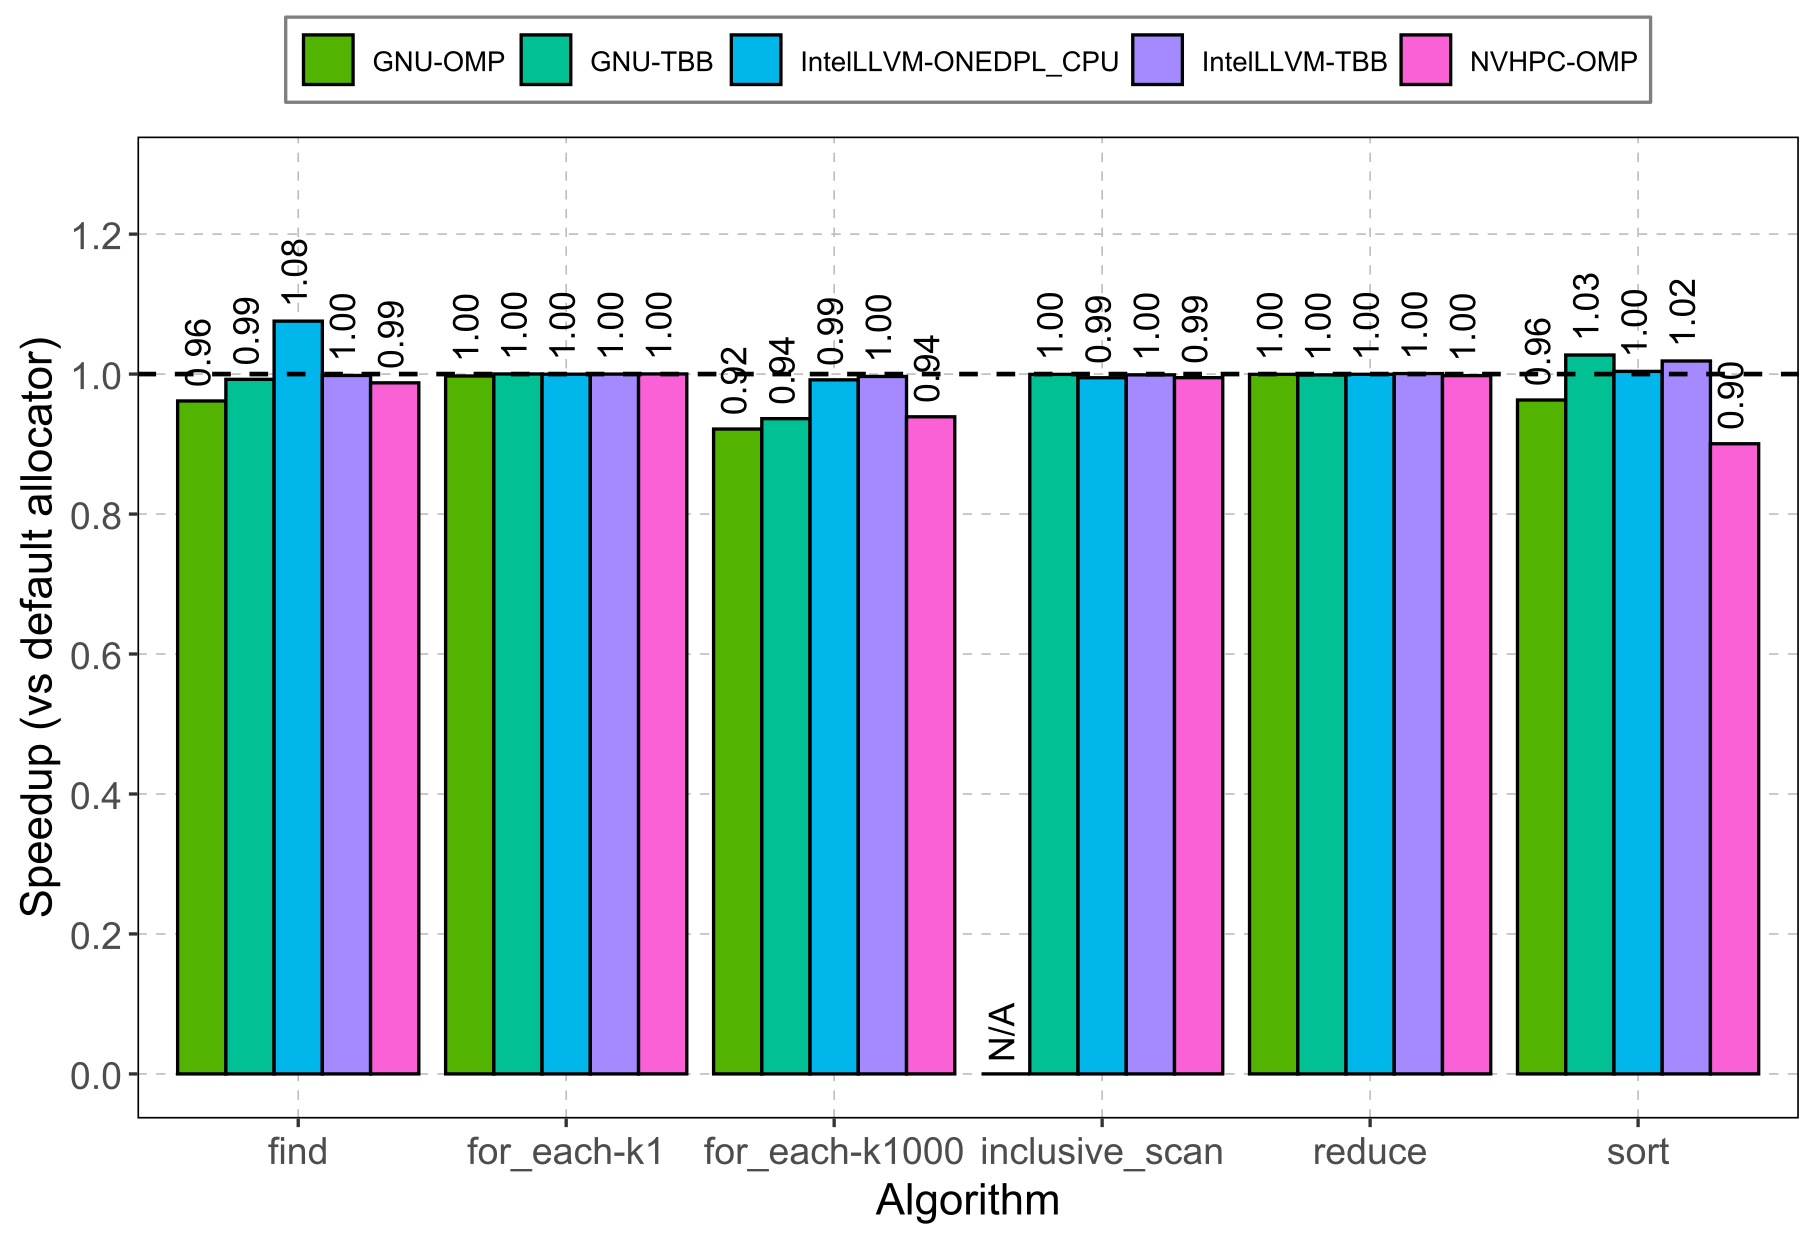
\includegraphics[width=\linewidth]{figures/speedup_customAllocator}
      \caption{Speedup when using custom parallel allocator with 32 threads and a problem size of $2^{29}$. Higher is better.}\label{fig:speedup_customAllocator}
\end{figure}

\subsection{X::for\_each}

This experiment evaluates the performance of the \textit{for\_each} algorithm.
The parameter \( k_{it} \) represents the arithmetic intensity of the workload,
specifically indicating how many times a computational operation is repeated
for each element of the input data. Thus, a higher \( k_{it} \) corresponds to
a more compute-intensive workload, and performance in this scenario is expected
to approach ideal speedup due to reduced relative overhead from
parallelization.

Figure~\ref{fig:problemSize_time-for_each} presents the execution times for
\textit{for\_each} using minimal and maximal arithmetic intensities,
represented by \( k_{it} \). The results closely resemble those reported in the
original pSTL-Bench paper. For the low-intensity case (\( k_{it} = 1 \)), the
NVIDIA OpenMP backend achieves the best performance. In contrast, for the
high-intensity scenario (\( k_{it} = 1000 \)), all backends exhibit similar
execution times.

The oneDPL backend on CPU consistently performed worse than the other backends
across both configurations.

\begin{figure}[H]
      \centering
      \begin{minipage}[t]{0.48\linewidth}
            \centering
            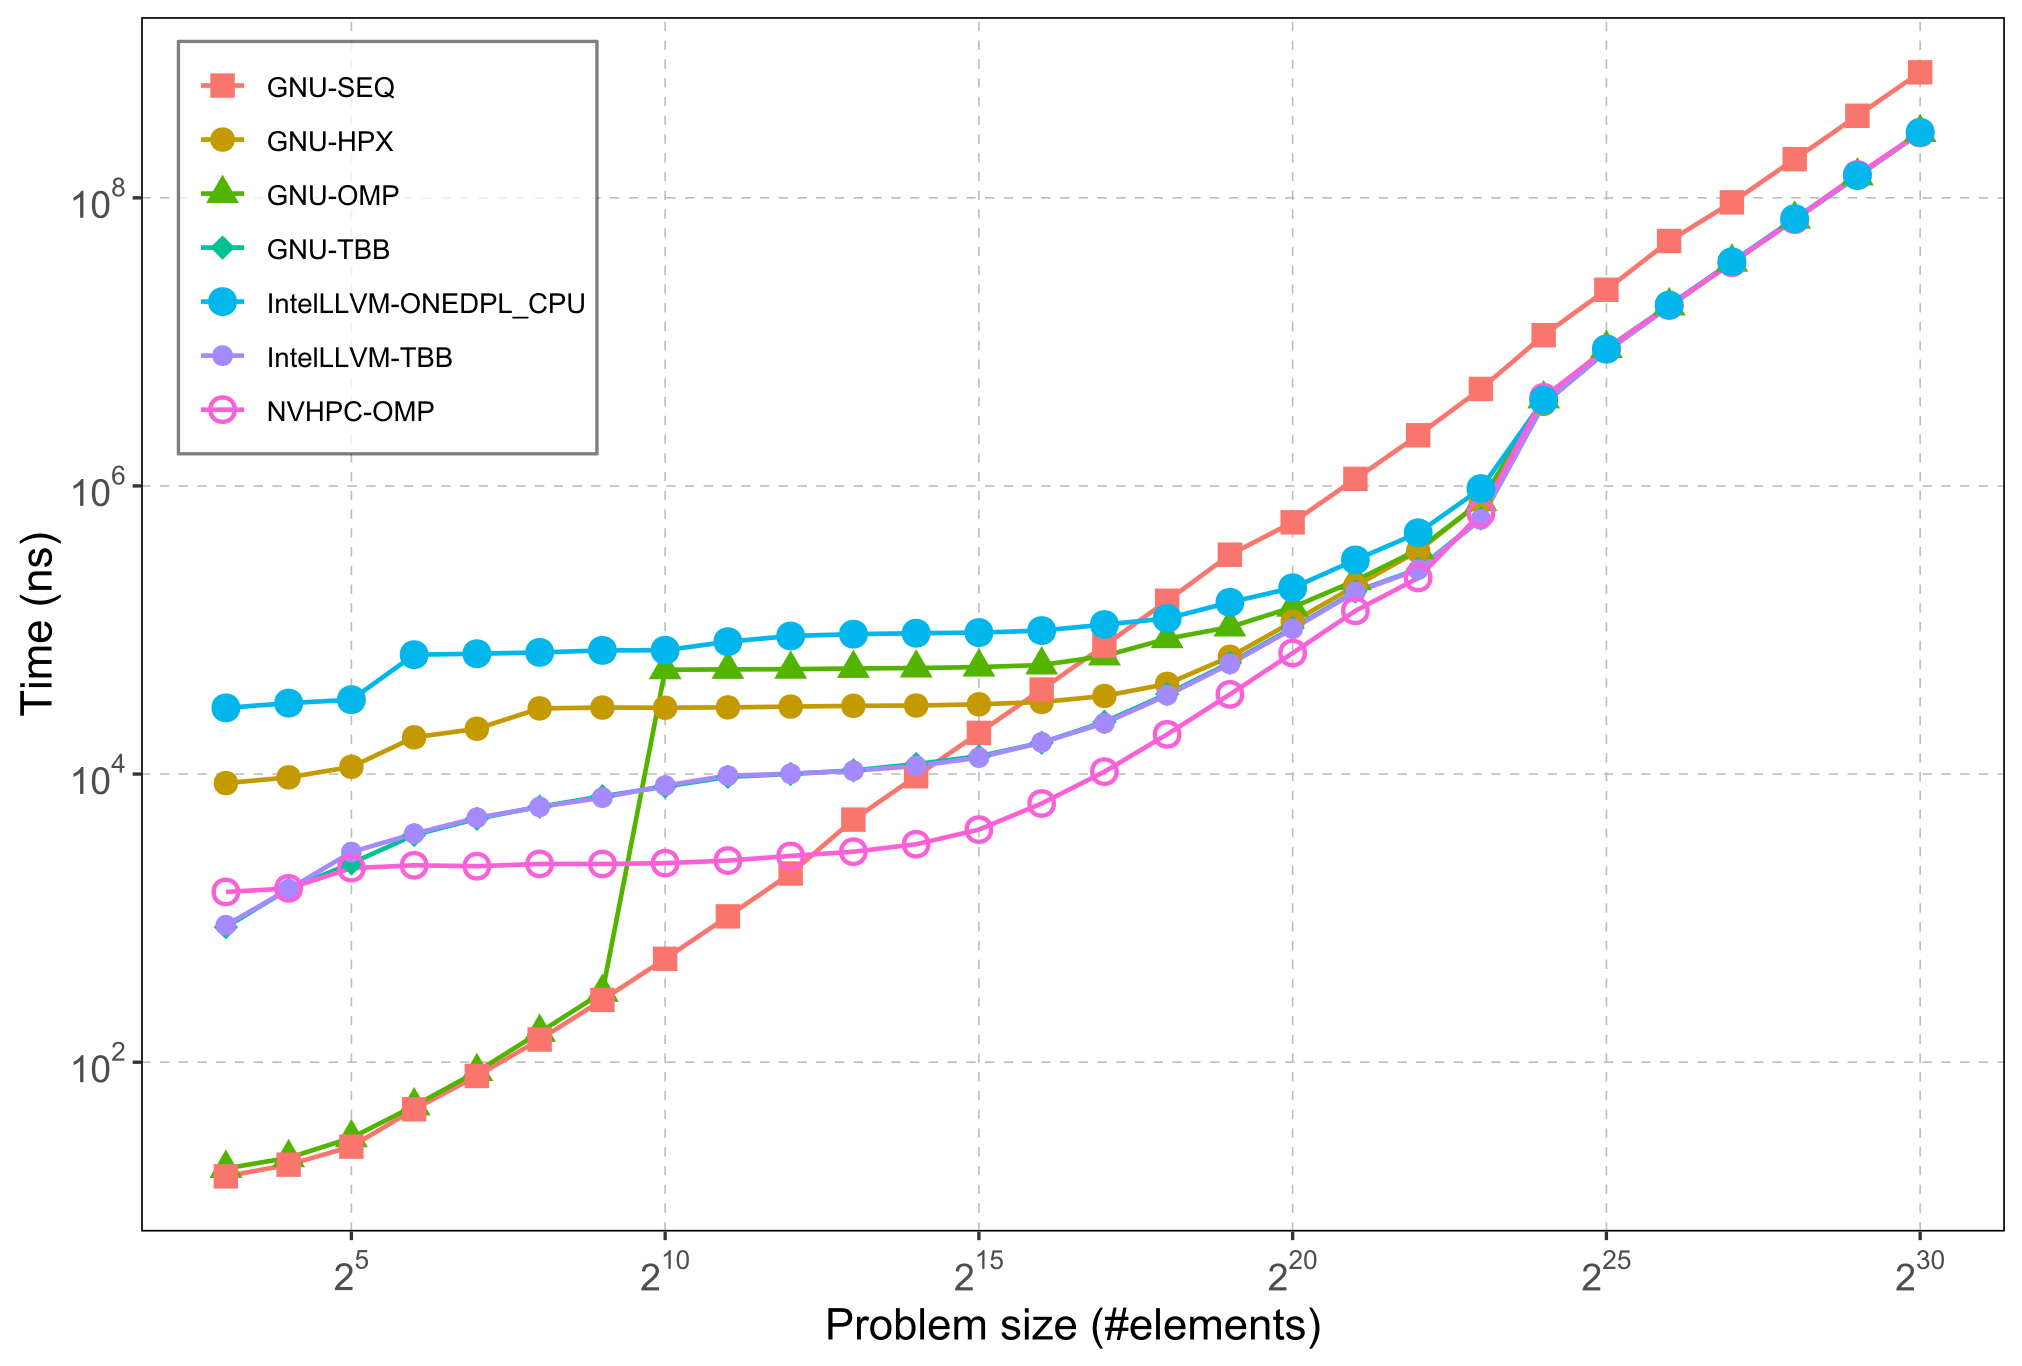
\includegraphics[width=\linewidth]{figures/problemSize_time-for_each-k1.png}
            \caption*{(a) $k_{it} = 1$.}
      \end{minipage}
      \hfill
      \begin{minipage}[t]{0.48\linewidth}
            \centering
            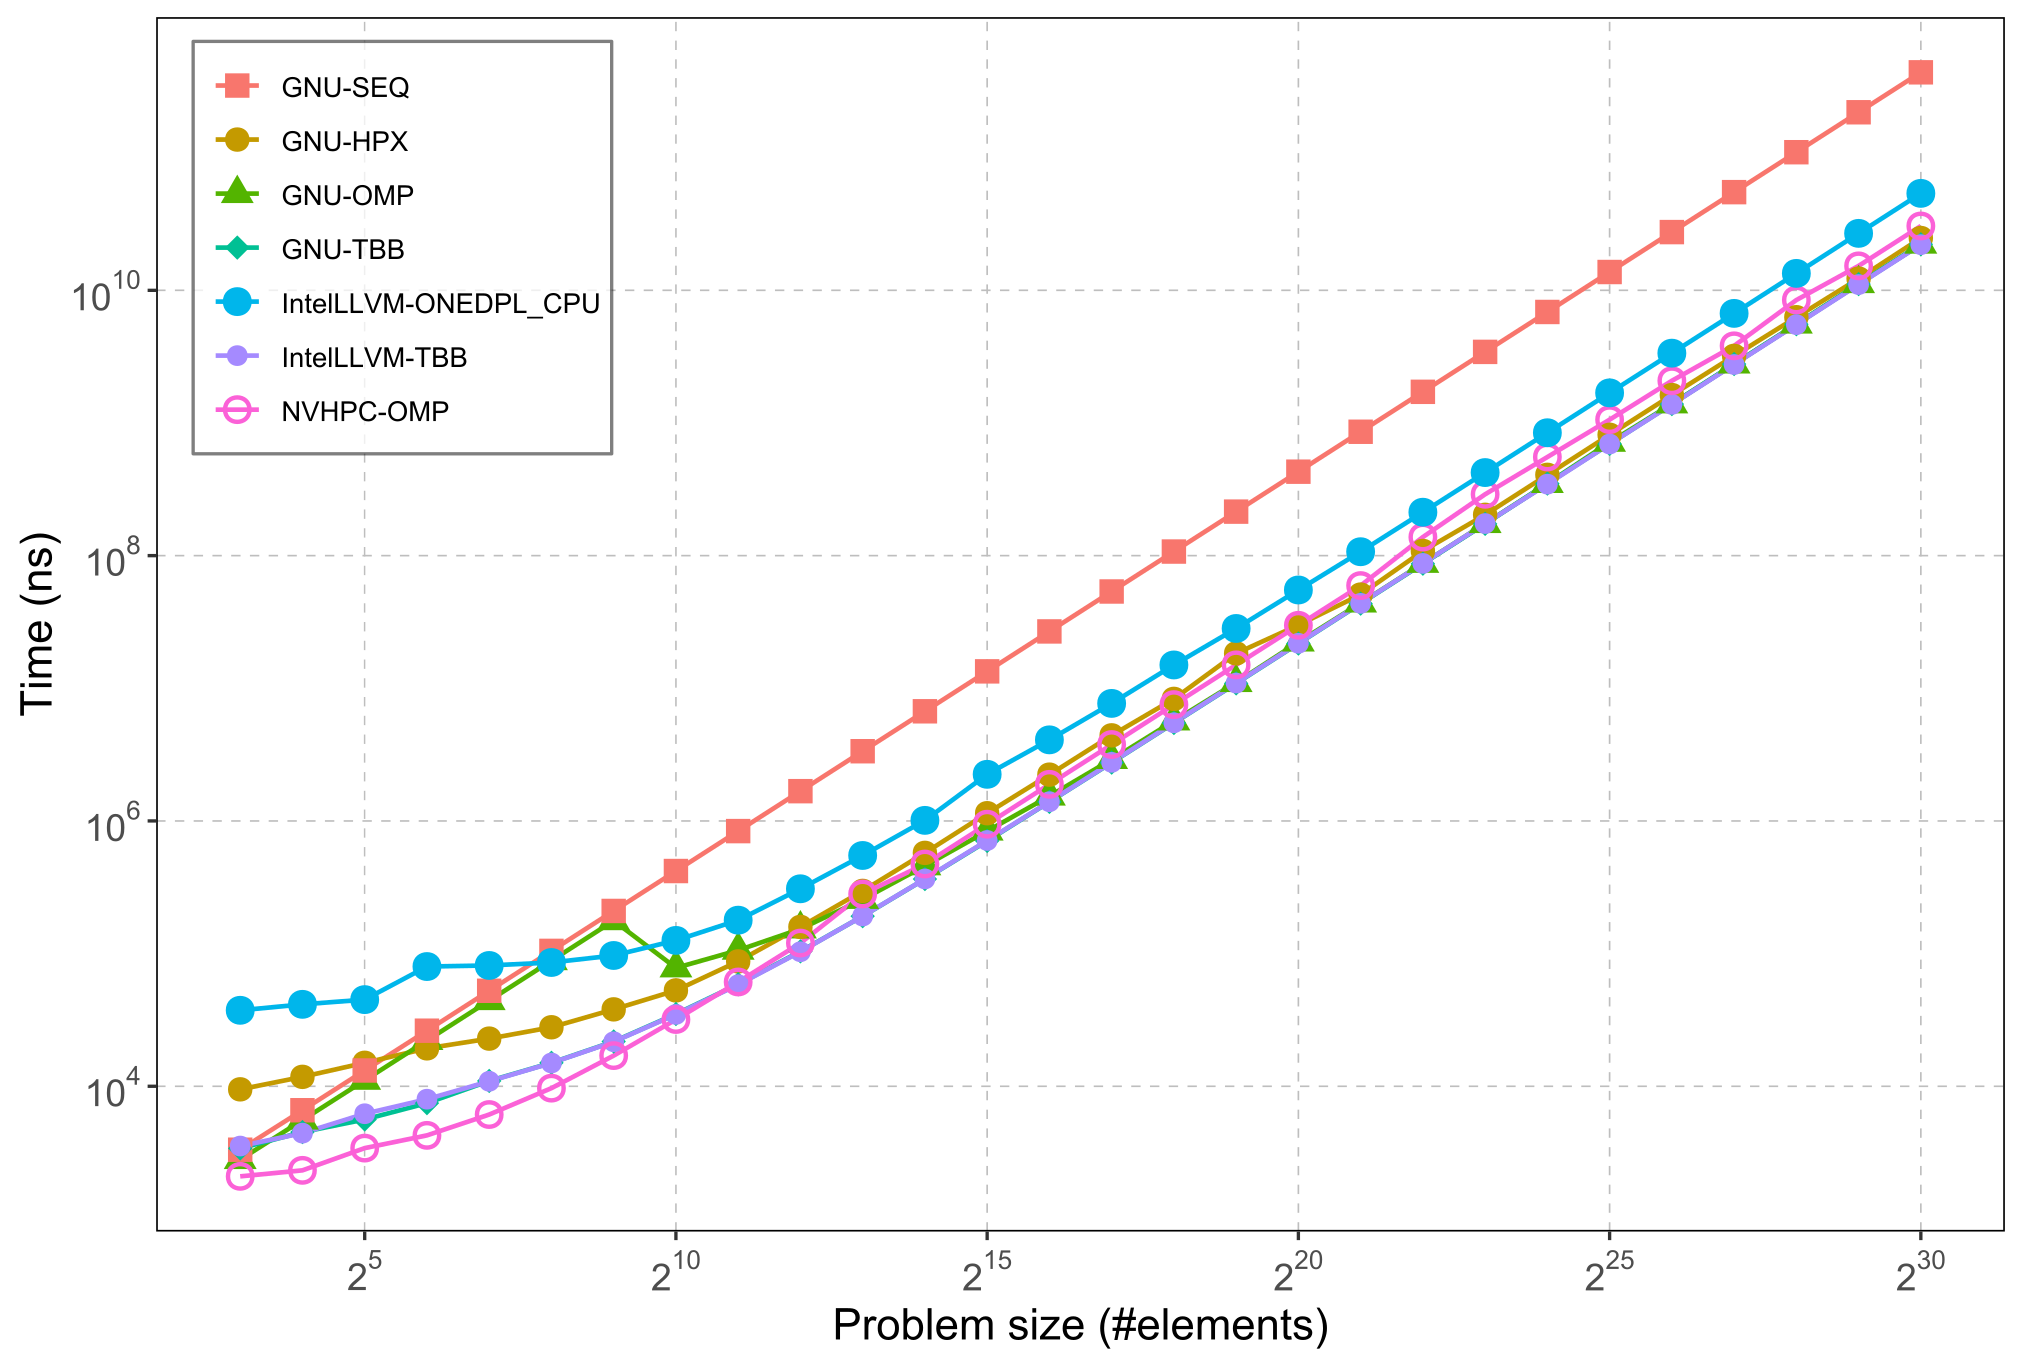
\includegraphics[width=\linewidth]{figures/problemSize_time-for_each-k1000.png}
            \caption*{(b) $k_{it} = 1000$.}
      \end{minipage}
      \caption{Results for benchmark X::for\_each. Problem size scaling using all
            cores except for the GNU-SEQ implementation. Lower is better.}
      \label{fig:problemSize_time-for_each}
\end{figure}

Figure~\ref{fig:speedup_threads-for_each} shows the strong scaling results for
the \textit{for\_each} algorithm with $2^{29}$ elements. Compared to the
original paper, the results differ slightly. In the original study, all
backends achieved ideal speedup for $k_{it} = 1000$ and near-ideal speedup for
$k_{it} = 1$.

In this evaluation, the oneDPL backend on CPU underperforms relative to the
others. Additionally, all backends begin to lose scalability beyond 8 threads,
which is likely due to the hardware architecture—specifically, the presence of
8 performance cores (P-cores) and 16 efficiency cores (E-cores).

\begin{figure}[H]
      \centering
      \begin{minipage}[t]{0.48\linewidth}
            \centering
            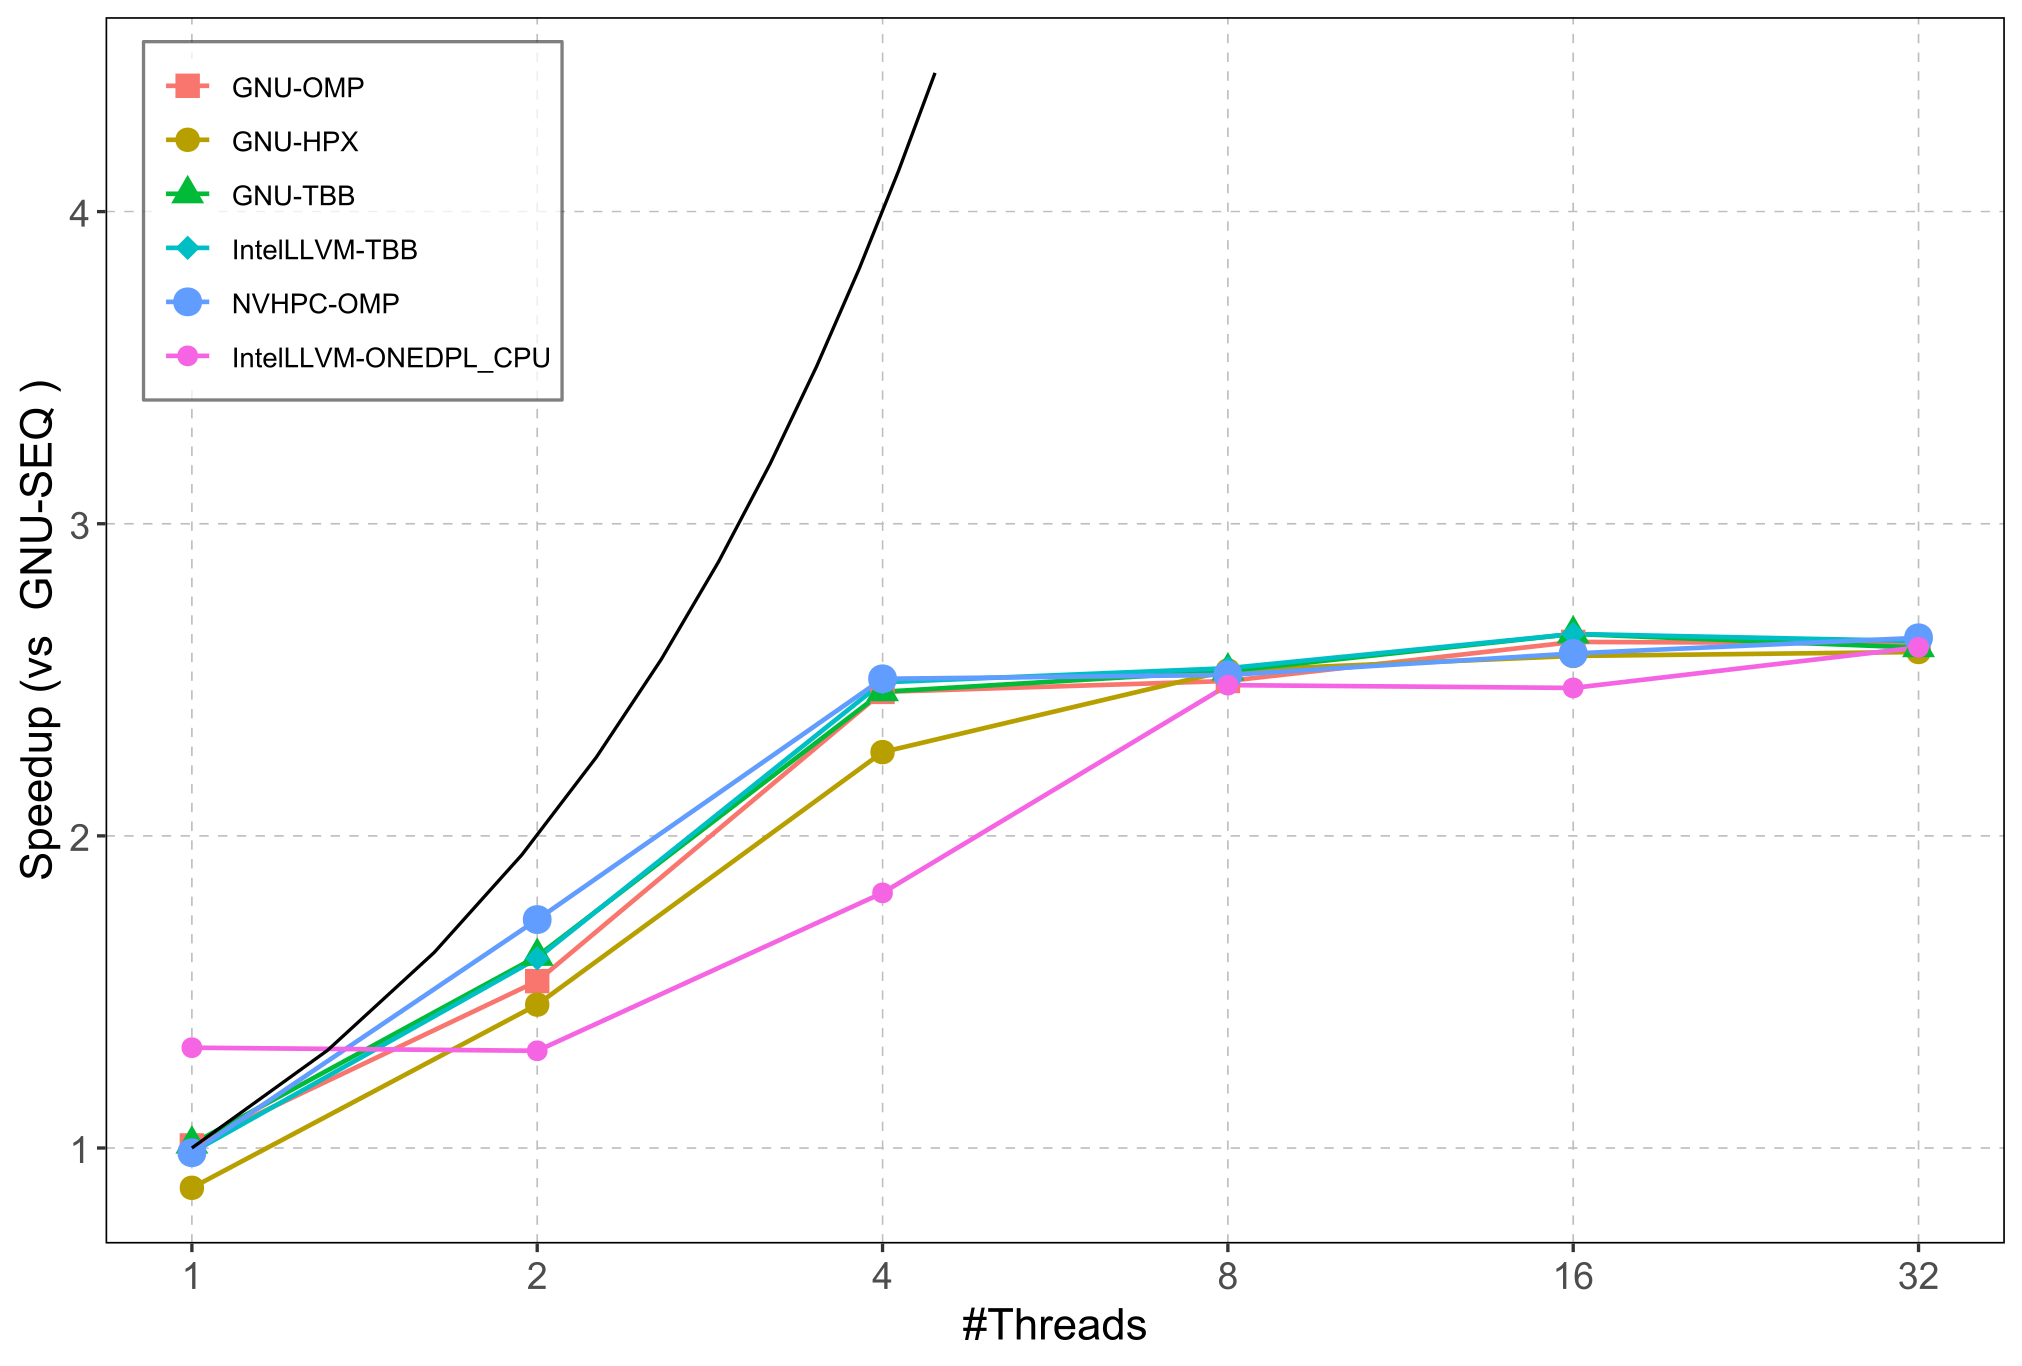
\includegraphics[width=\linewidth]{figures/speedup_threads-for_each-k1.png}
            \caption*{(a) $k_{it} = 1$.}
      \end{minipage}
      \hfill
      \begin{minipage}[t]{0.48\linewidth}
            \centering
            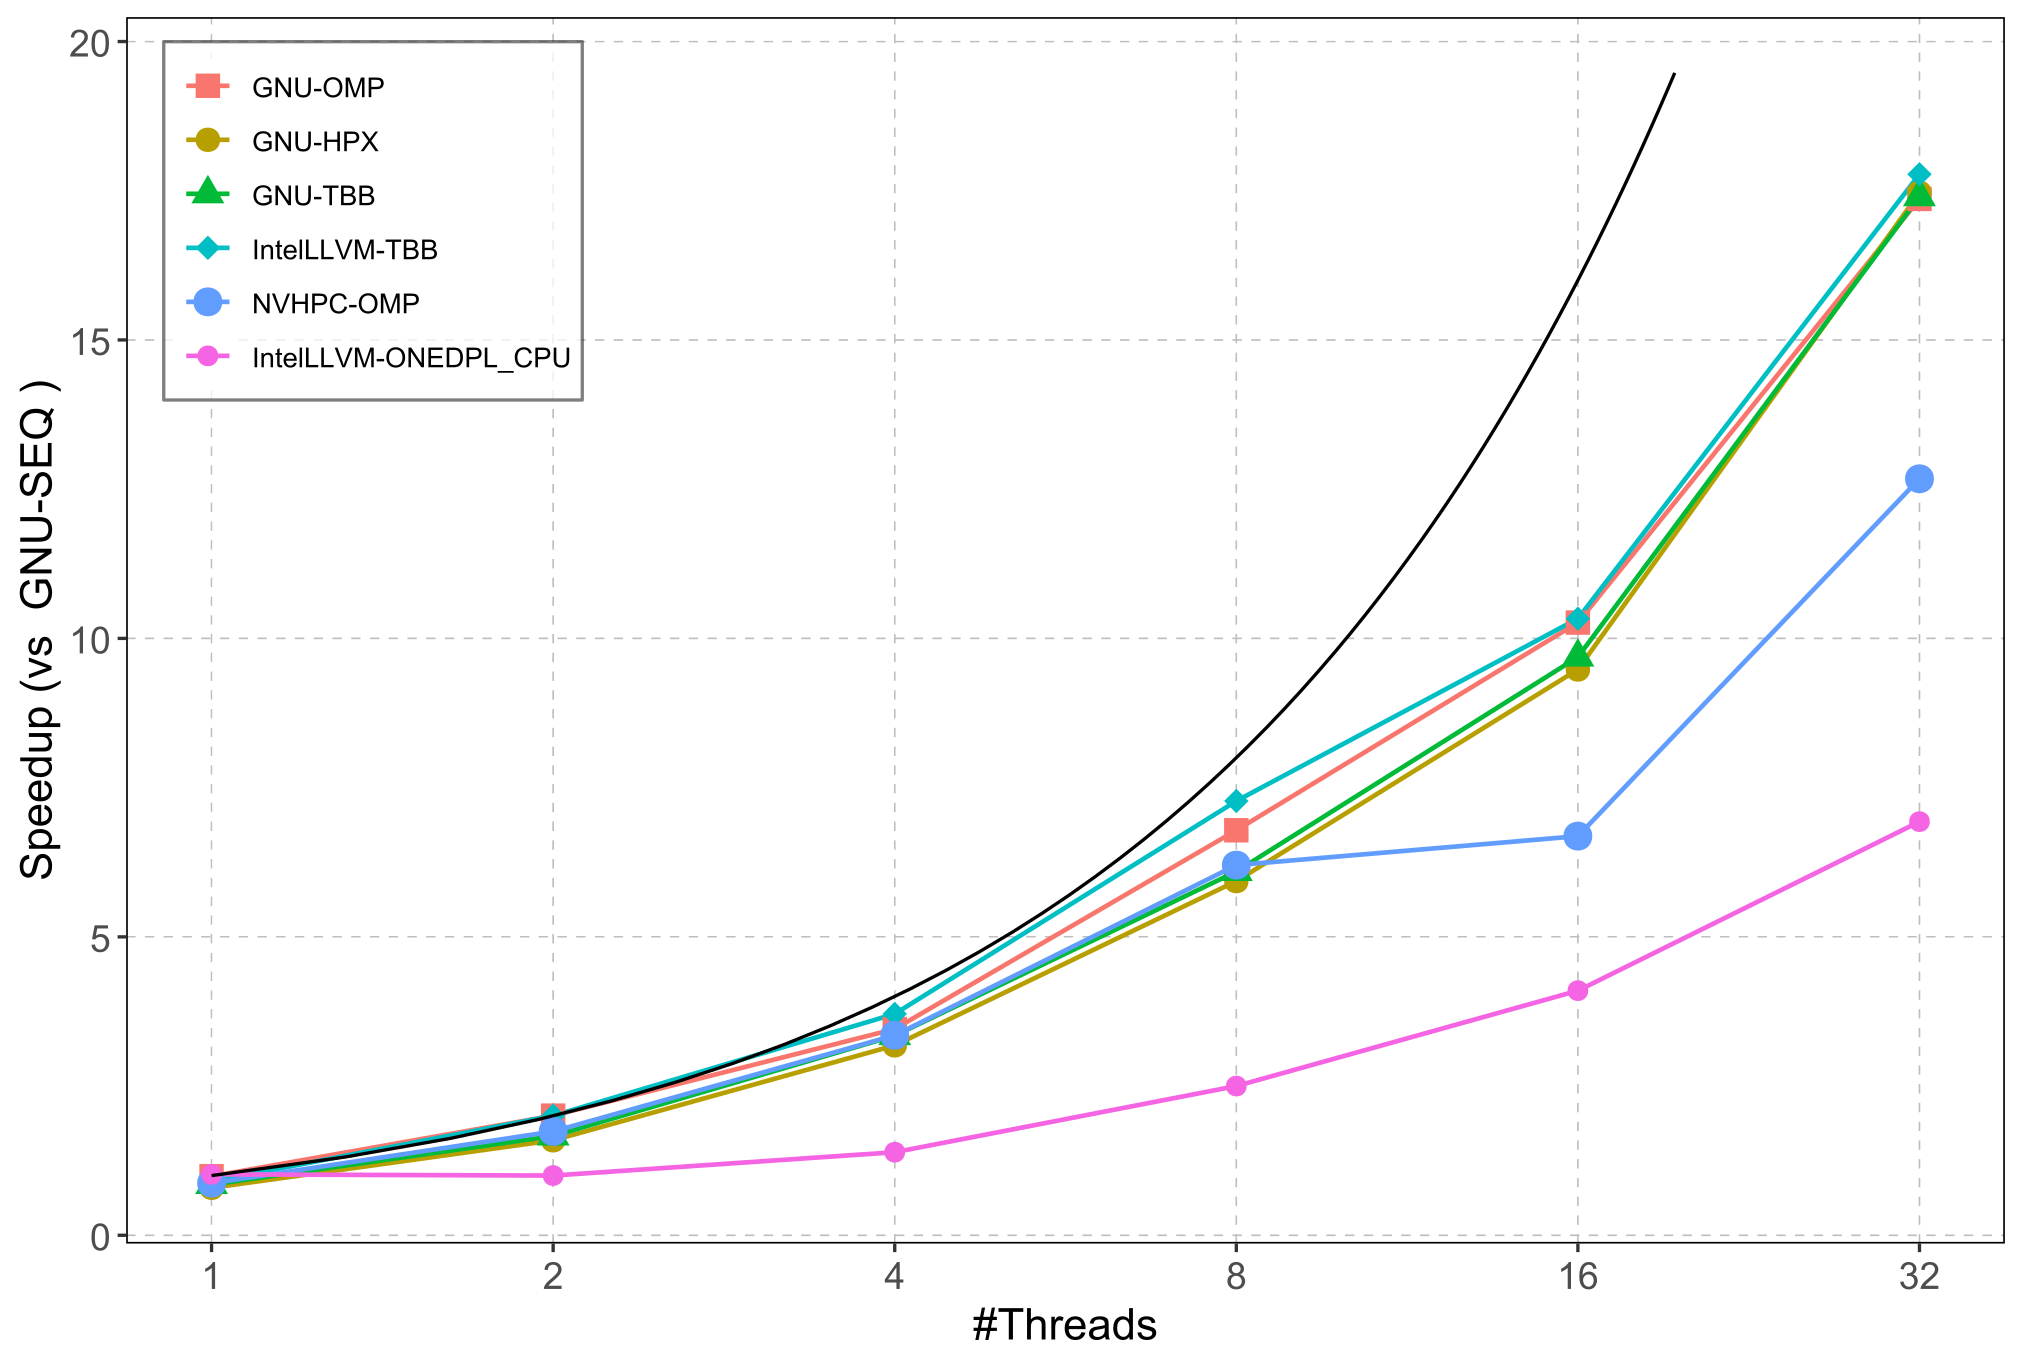
\includegraphics[width=\linewidth]{figures/speedup_threads-for_each-k1000.png}
            \caption*{(b) $k_{it} = 1000$.}
      \end{minipage}
      \caption{Results for benchmark X::for\_each. Strong scaling with $2^{29}$
            elements. Higher is better.}\label{fig:speedup_threads-for_each}
\end{figure}

\subsection{X::find}
The \textit{find} algorithm performs a linear search over a range to locate a
target value.

Figure~\ref{fig:x::find} presents the execution time and speedup for the
\textit{find} algorithm. The results are consistent with those reported in the
original pSTL-Bench paper, where sequential execution significantly outperforms
parallel implementations for small problem sizes.

As the problem size increases, parallel backends gradually begin to outperform
the sequential version.

However, the maximum observed speedup remains relatively modest, with the best
performance achieved by the NVIDIA OpenMP backend.

Across all problem sizes, the oneDPL backend on CPU consistently delivered the
worst performance.

\begin{figure}[H]
      \centering
      \begin{minipage}[t]{0.48\linewidth}
            \centering
            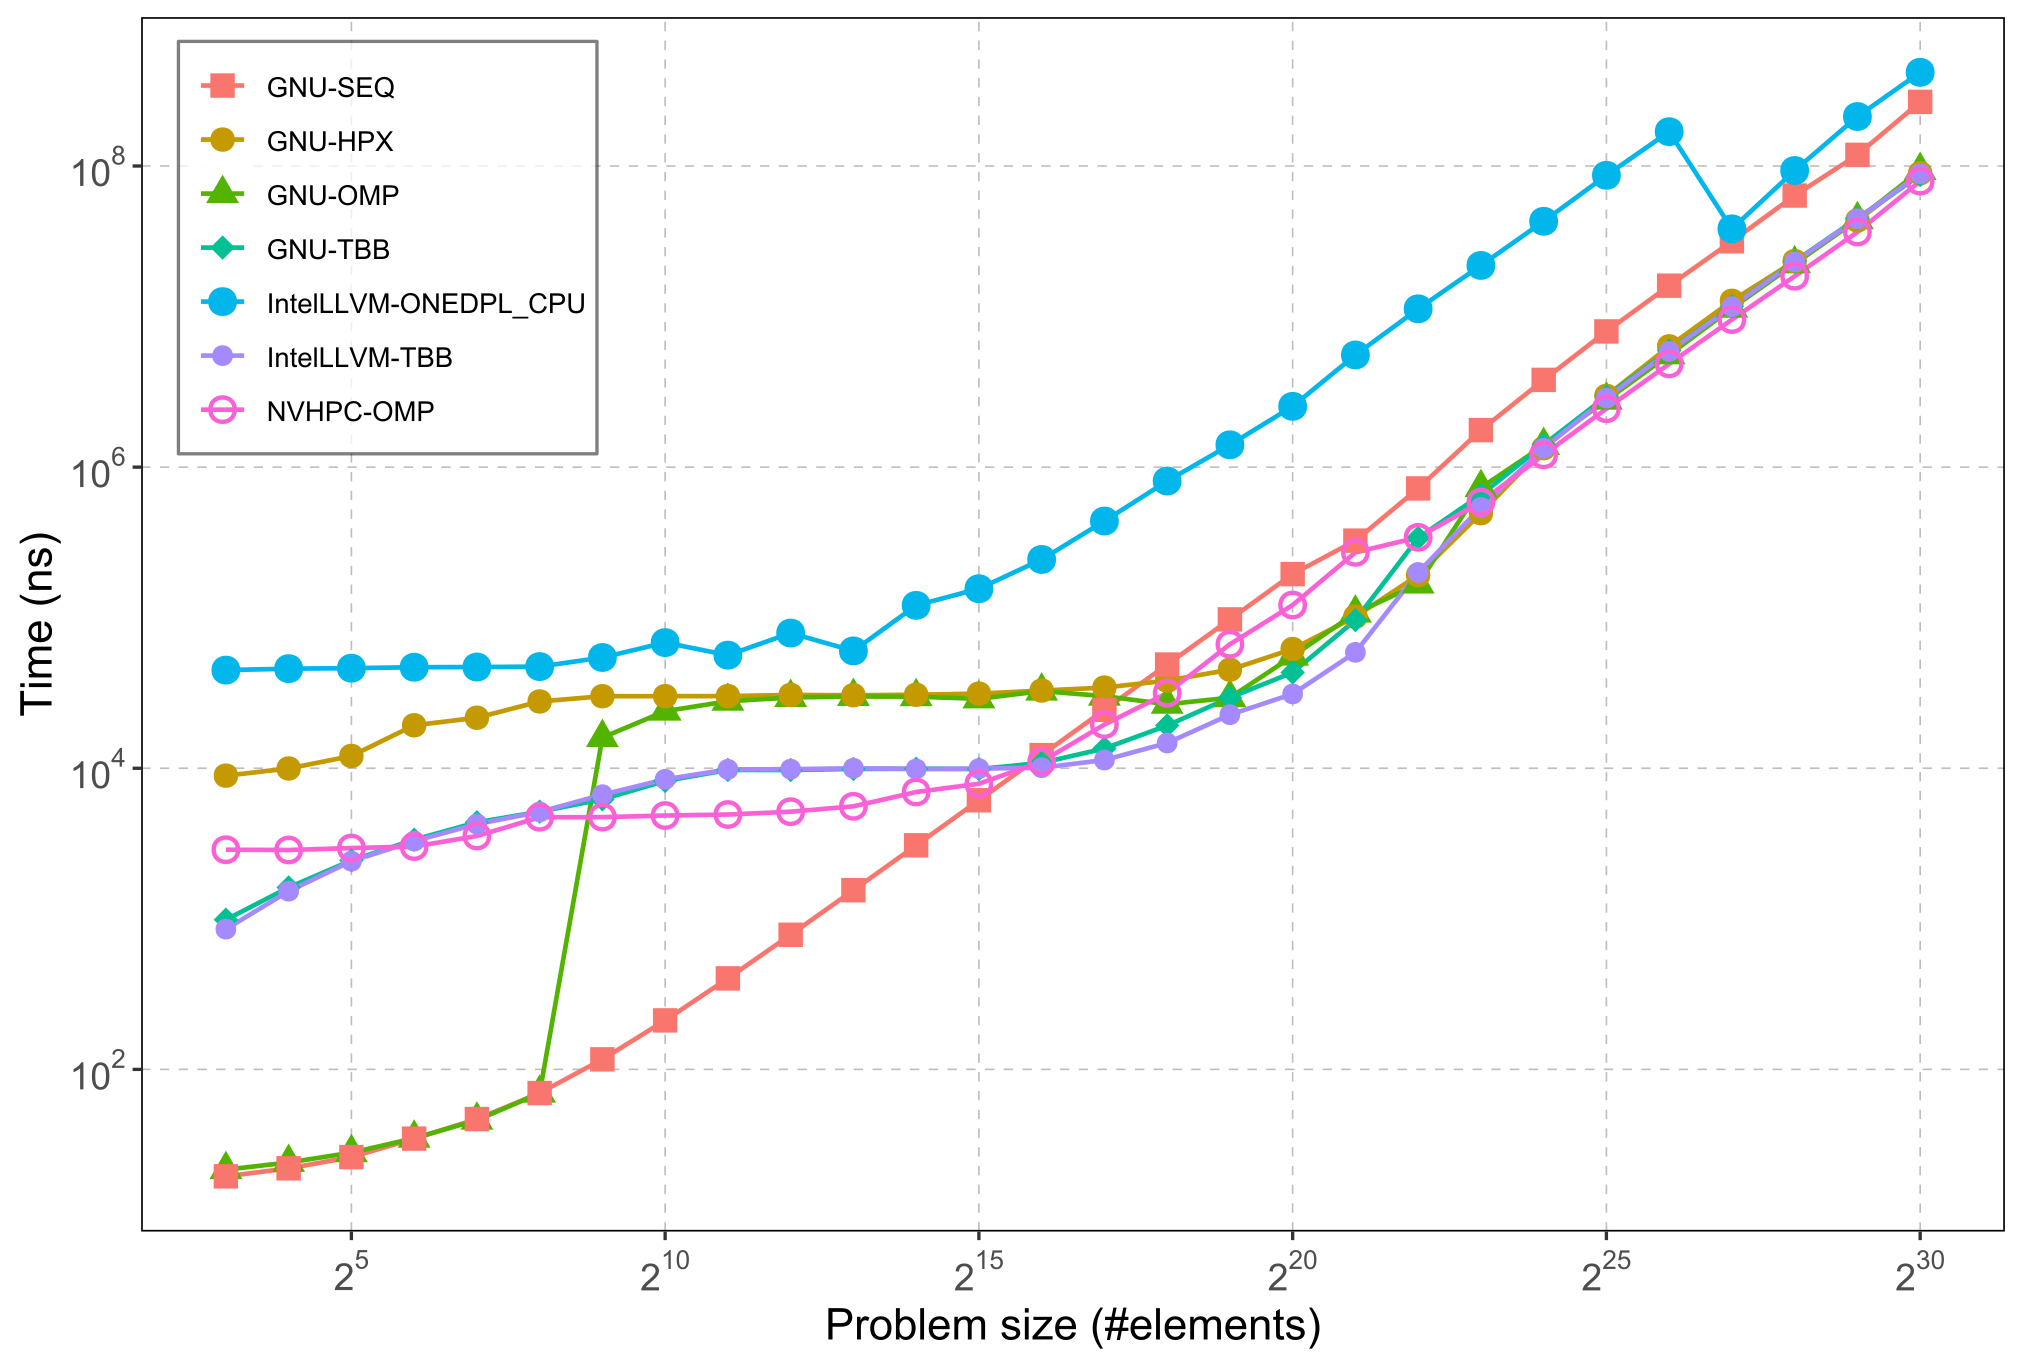
\includegraphics[width=\linewidth]{figures/problemSize_time-find.png}
            \caption*{(a) Problem scaling. Lower is better.}
      \end{minipage}
      \hfill
      \begin{minipage}[t]{0.48\linewidth}
            \centering
            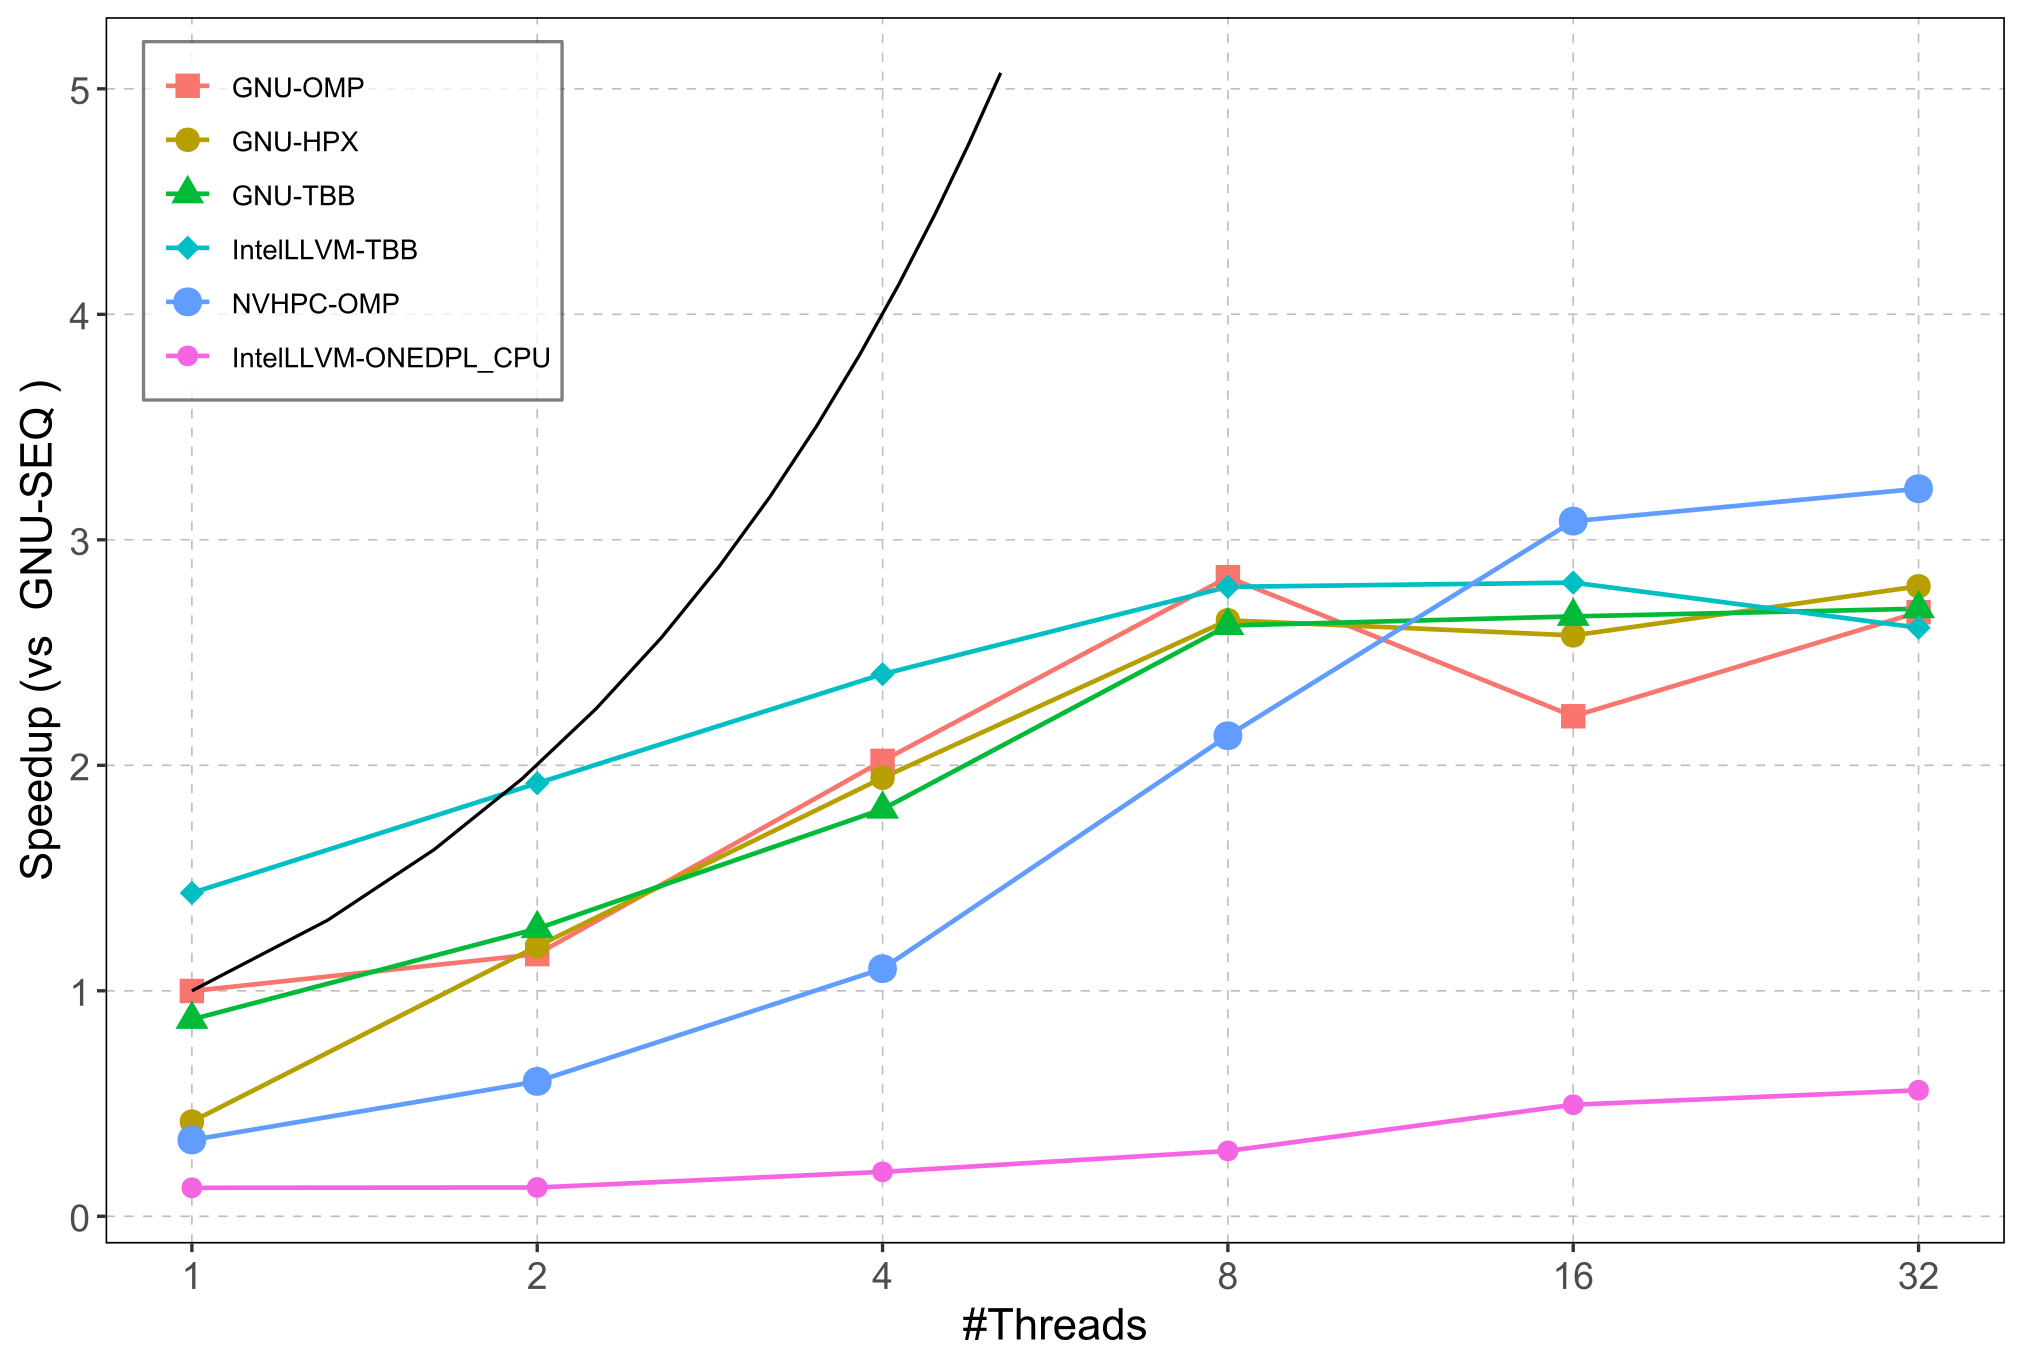
\includegraphics[width=\linewidth]{figures/speedup_threads-find.png}
            \caption*{(b) Strong scaling with $2^{29}$ elements. Higher is better.}
      \end{minipage}
      \caption{Results for X::find.}\label{fig:x::find}
\end{figure}

\subsection{X::inclusive\_scan}

The \textit{inclusive\_scan} algorithm computes a prefix sum, where each
element in the output is the sum of all preceding elements plus the current
element.

The GNU OpenMP implementation is omitted from the results, as it does not
support this algorithm. Although the NVIDIA OpenMP backend also lacks native
support, it falls back to a sequential implementation.

Figure~\ref{fig:x::inclusive_scan} shows the execution time and speedup for the
\textit{inclusive\_scan} algorithm. The results are consistent with those in
the original pSTL-Bench paper, where sequential execution significantly
outperforms parallel implementations for small problem sizes.

As the problem size increases, the performance of the parallel backends begins
to approach that of the sequential version, with the TBB implementations
achieving the best results overall.

Observed speedups remain modest and tend to degrade when using more than 8
threads. This decline is likely due to the underlying hardware architecture,
which consists of 8 performance cores (P-cores) and 16 efficiency cores
(E-cores).

Across all problem sizes, the oneDPL backend on CPU consistently exhibited the
lowest performance—even falling below that of the sequential baseline.

\begin{figure}[H]
      \centering
      \begin{minipage}[t]{0.48\linewidth}
            \centering
            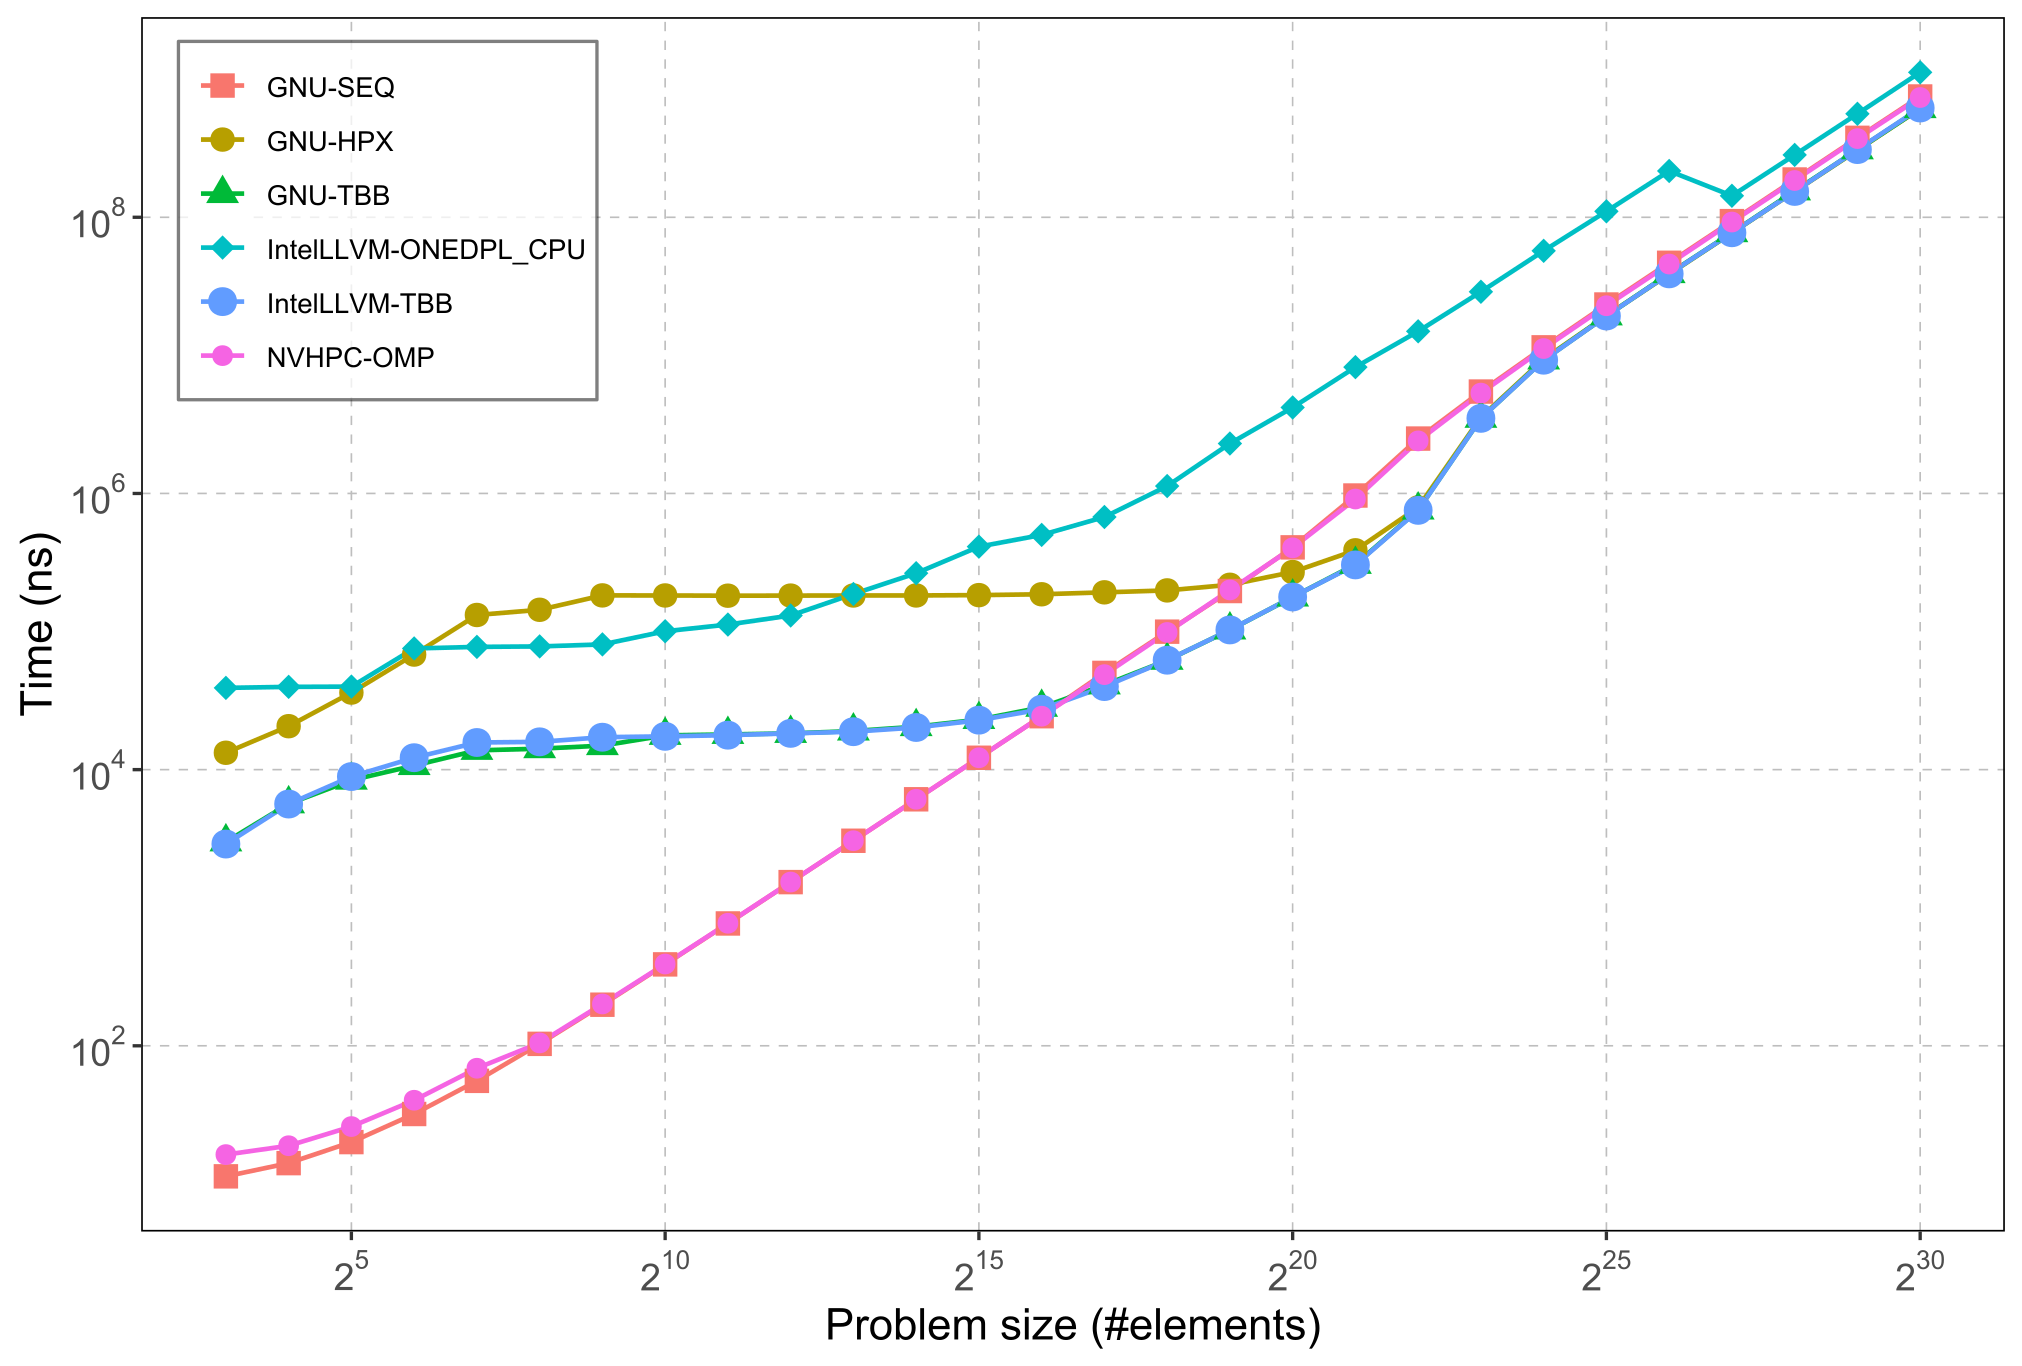
\includegraphics[width=\linewidth]{figures/problemSize_time-inclusive_scan.png}
            \caption*{(a) Problem scaling. Lower is better.}
      \end{minipage}
      \hfill
      \begin{minipage}[t]{0.48\linewidth}
            \centering
            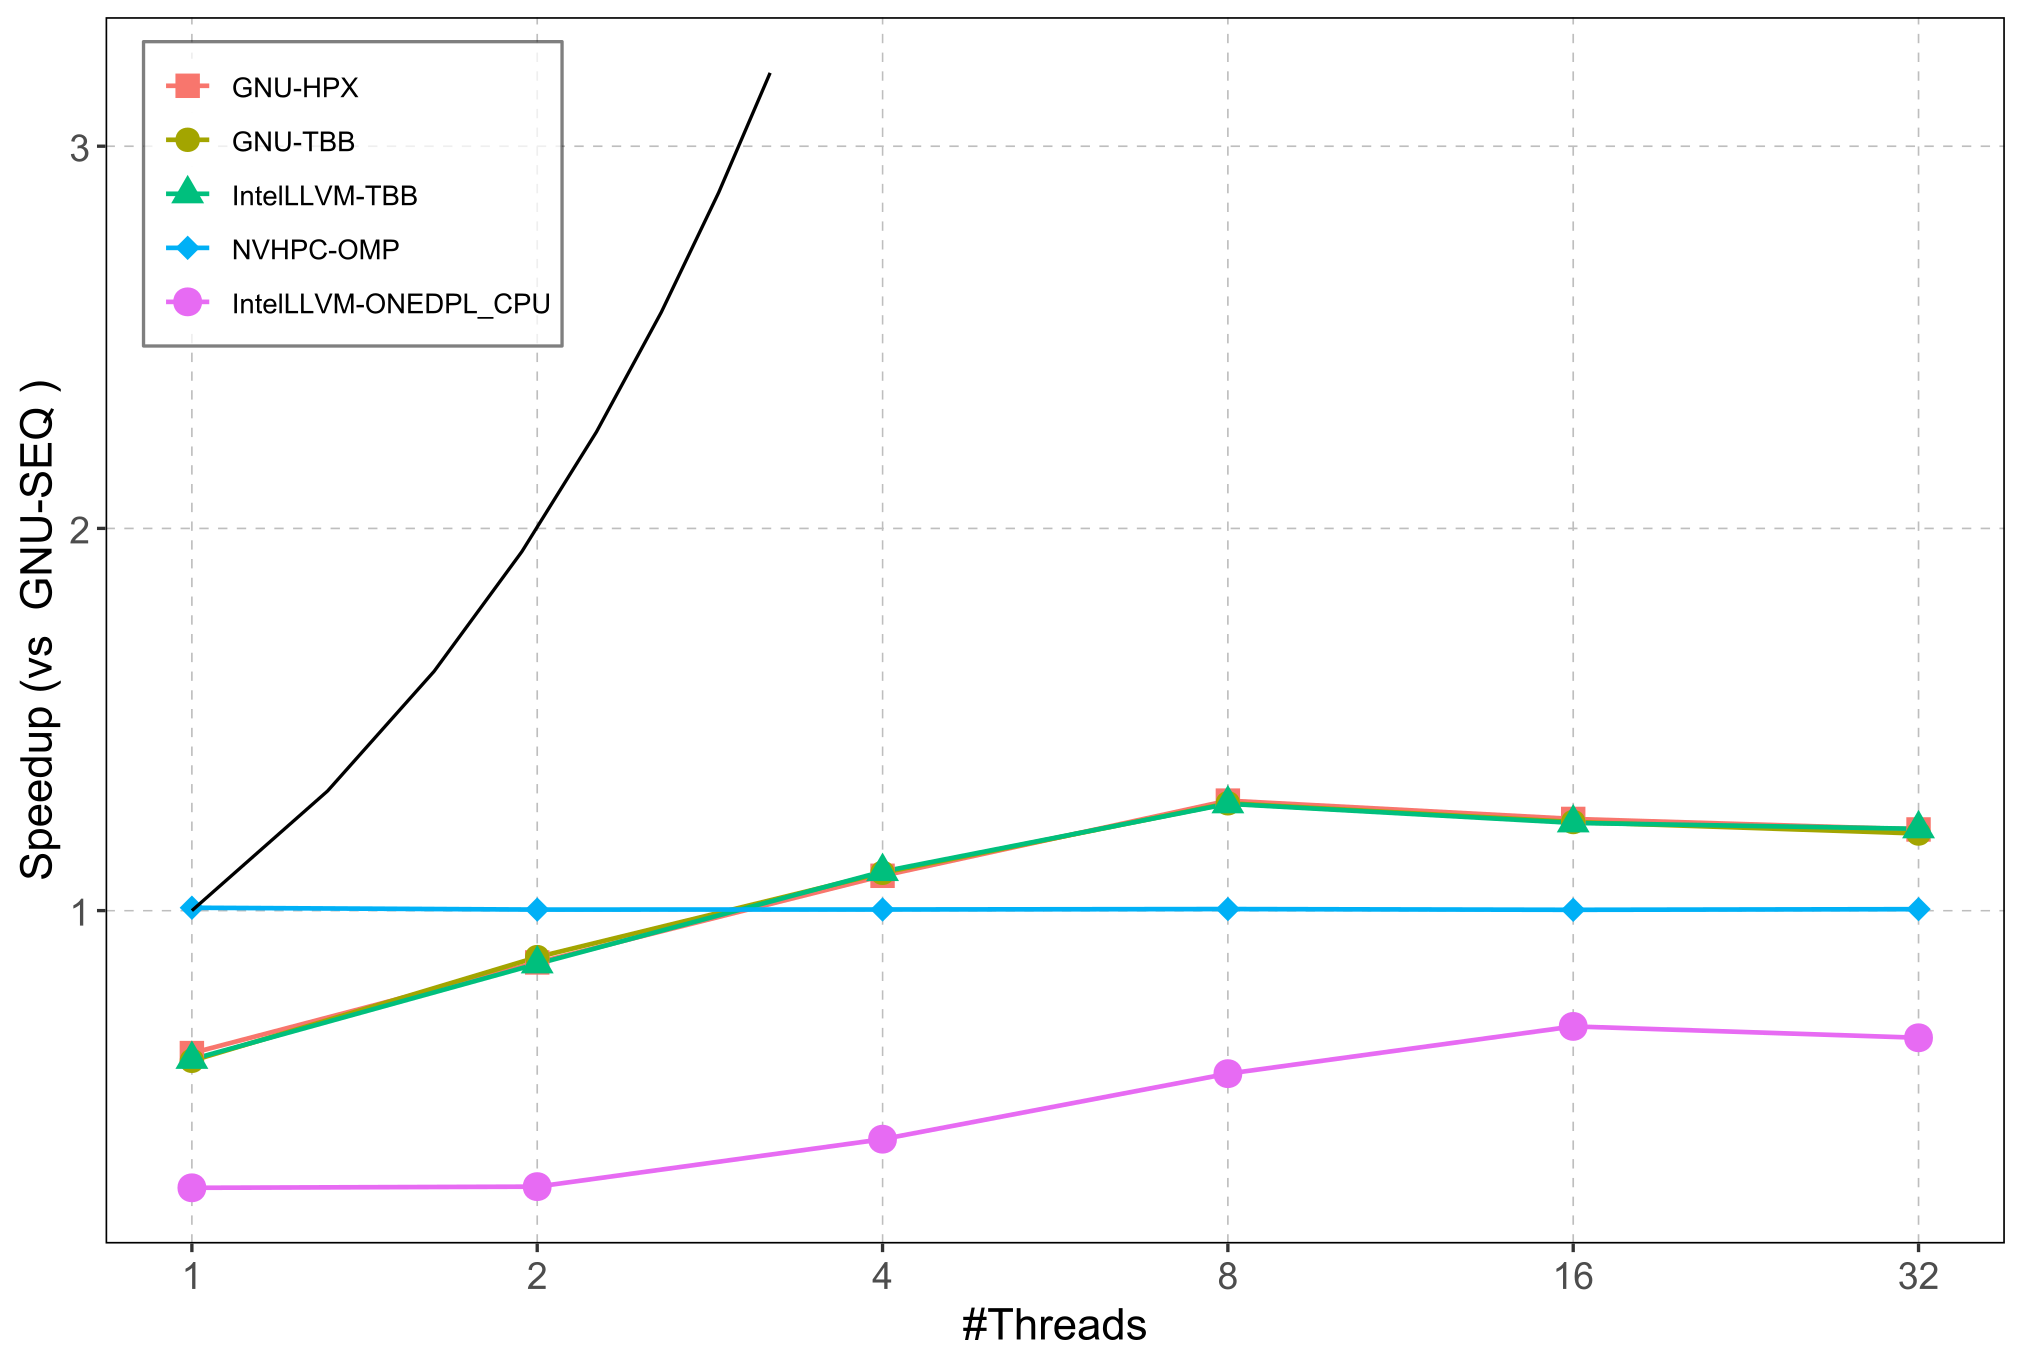
\includegraphics[width=\linewidth]{figures/speedup_threads-inclusive_scan.png}
            \caption*{(b) Strong scaling with $2^{29}$ elements. Higher is better.}
      \end{minipage}
      \caption{Results for X::inclusive\_scan.}\label{fig:x::inclusive_scan}
\end{figure}

\subsection{X::reduce}
The \textit{reduce} algorithm computes a single result by summing all elements
in a given range.

Figure~\ref{fig:x::reduce} presents the execution time and speedup for the
\textit{reduce} algorithm.

Sequential execution significantly outperforms parallel implementations for
small problem sizes. However, as the problem size increases, parallel backends
begin to surpass the sequential version in performance.

At a problem size of $2^{17}$ elements, most backends reach performance levels
comparable to the sequential baseline, with the exception of the oneDPL backend
on CPU, which achieves similar performance only at $2^{27}$ elements and
beyond.

The maximum observed speedup is typically reached at 8 threads for most
backends. Beyond this point, performance begins to degrade, likely due to the
limitations of the underlying hardware architecture.

\begin{figure}[H]
      \centering
      \begin{minipage}[t]{0.48\linewidth}
            \centering
            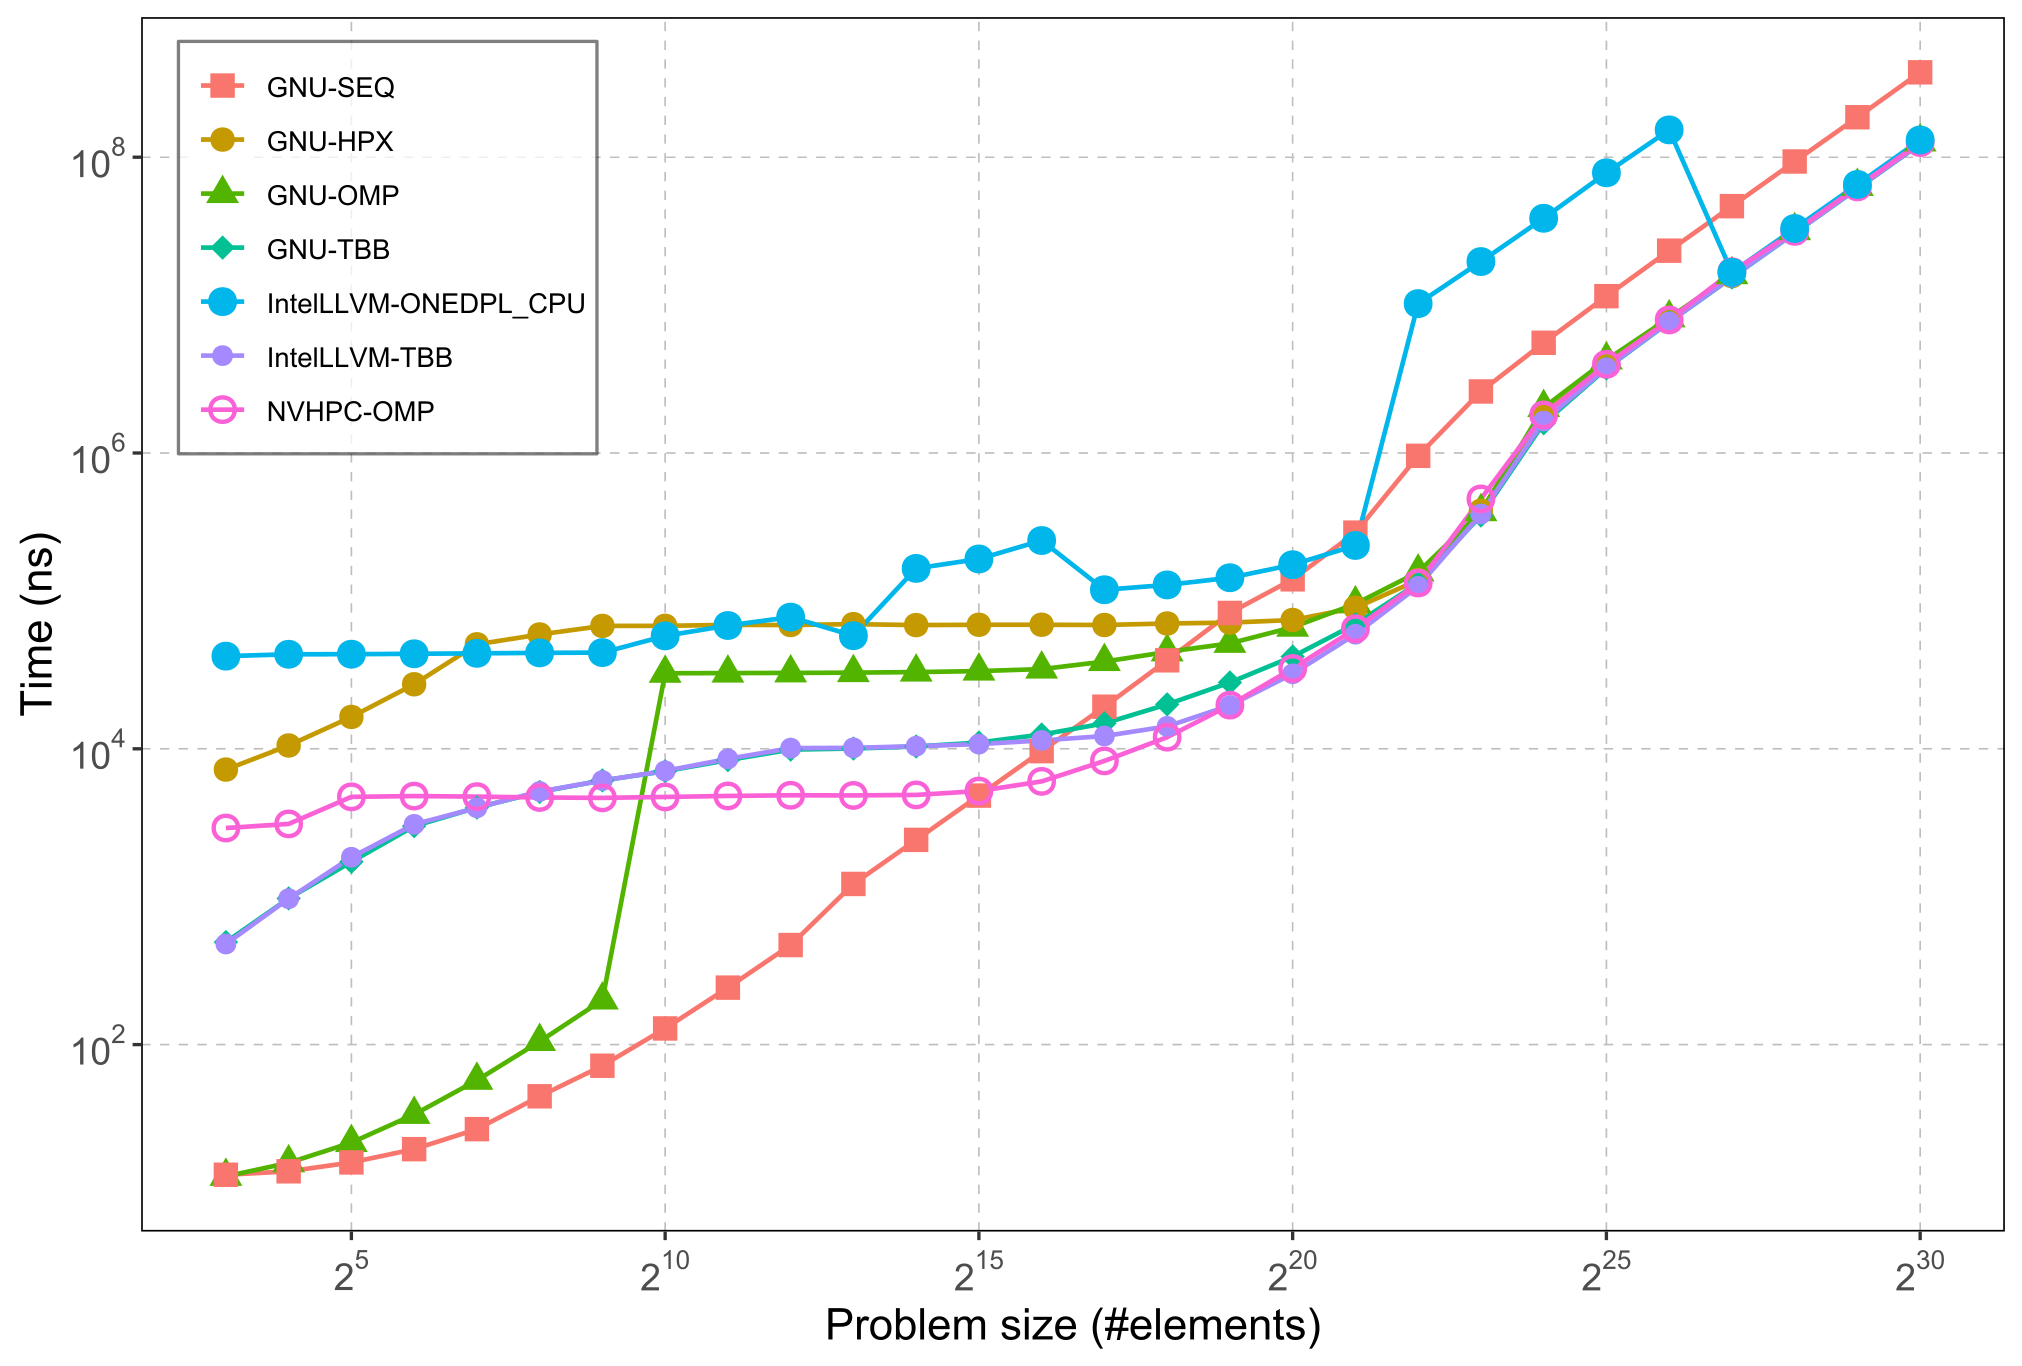
\includegraphics[width=\linewidth]{figures/problemSize_time-reduce.png}
            \caption*{(a) Problem scaling. Lower is better.}
      \end{minipage}
      \hfill
      \begin{minipage}[t]{0.48\linewidth}
            \centering
            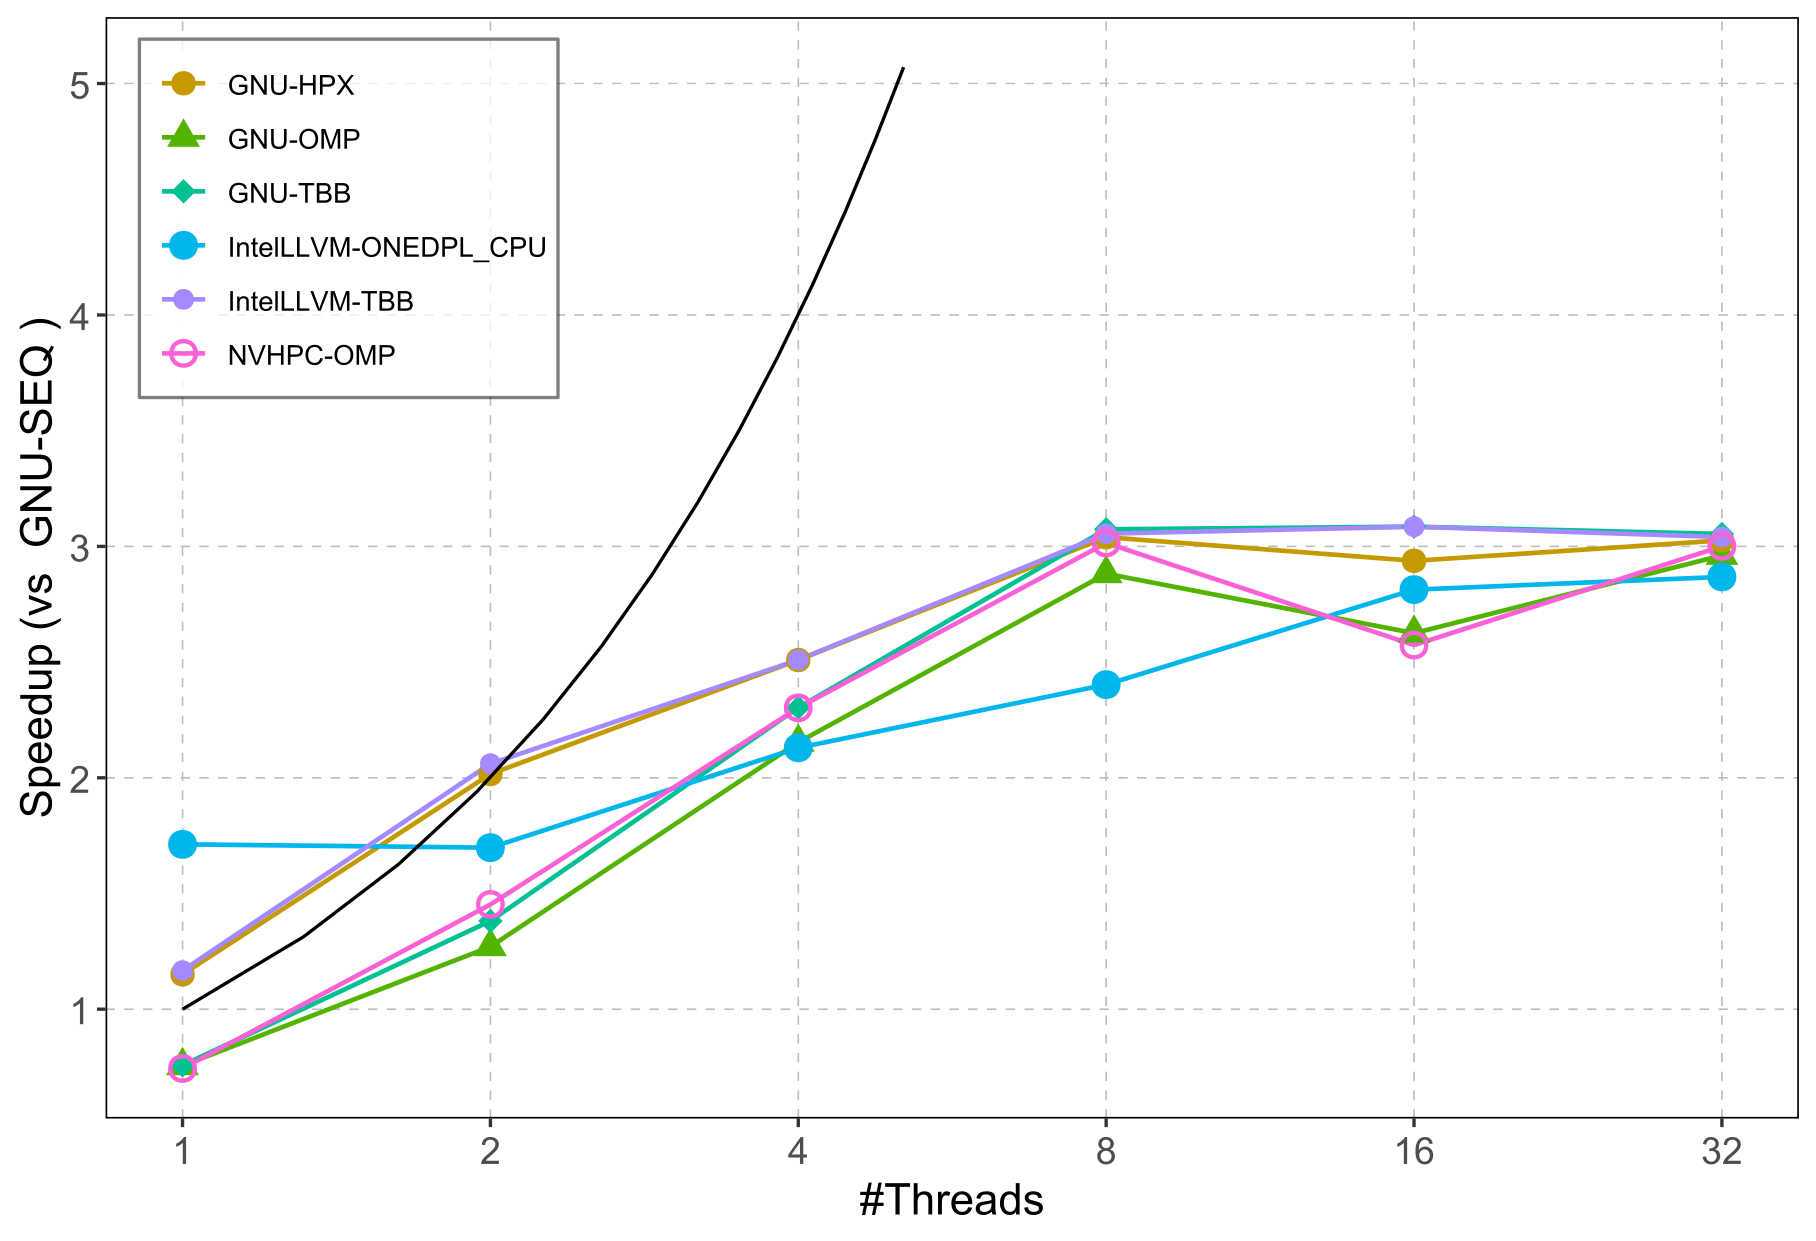
\includegraphics[width=\linewidth]{figures/speedup_threads-reduce.png}
            \caption*{(b) Strong scaling with $2^{29}$ elements. Higher is better.}
      \end{minipage}
      \caption{Results for X::reduce.}\label{fig:x::reduce}
\end{figure}

\subsection{X::sort}
The \textit{sort} algorithm rearranges elements in ascending order.

Figure~\ref{fig:x::sort} presents the execution time for the \textit{sort}
algorithm.

The results are consistent with those reported in the original pSTL-Bench
paper. The NVIDIA OpenMP backend achieves the best performance for small
problem sizes, while the GNU OpenMP backend performs best at larger scales.

Among all backends, only GNU OpenMP achieves near-ideal speedup. In contrast,
the others exhibit diminishing returns as the number of threads increases.

The oneDPL backend on CPU ranks among the weakest in the problem size scaling
experiment and performs the worst in the strong scaling scenario, falling
significantly short of ideal speedup.

\begin{figure}[H]
      \centering
      \begin{minipage}[t]{0.48\linewidth}
            \centering
            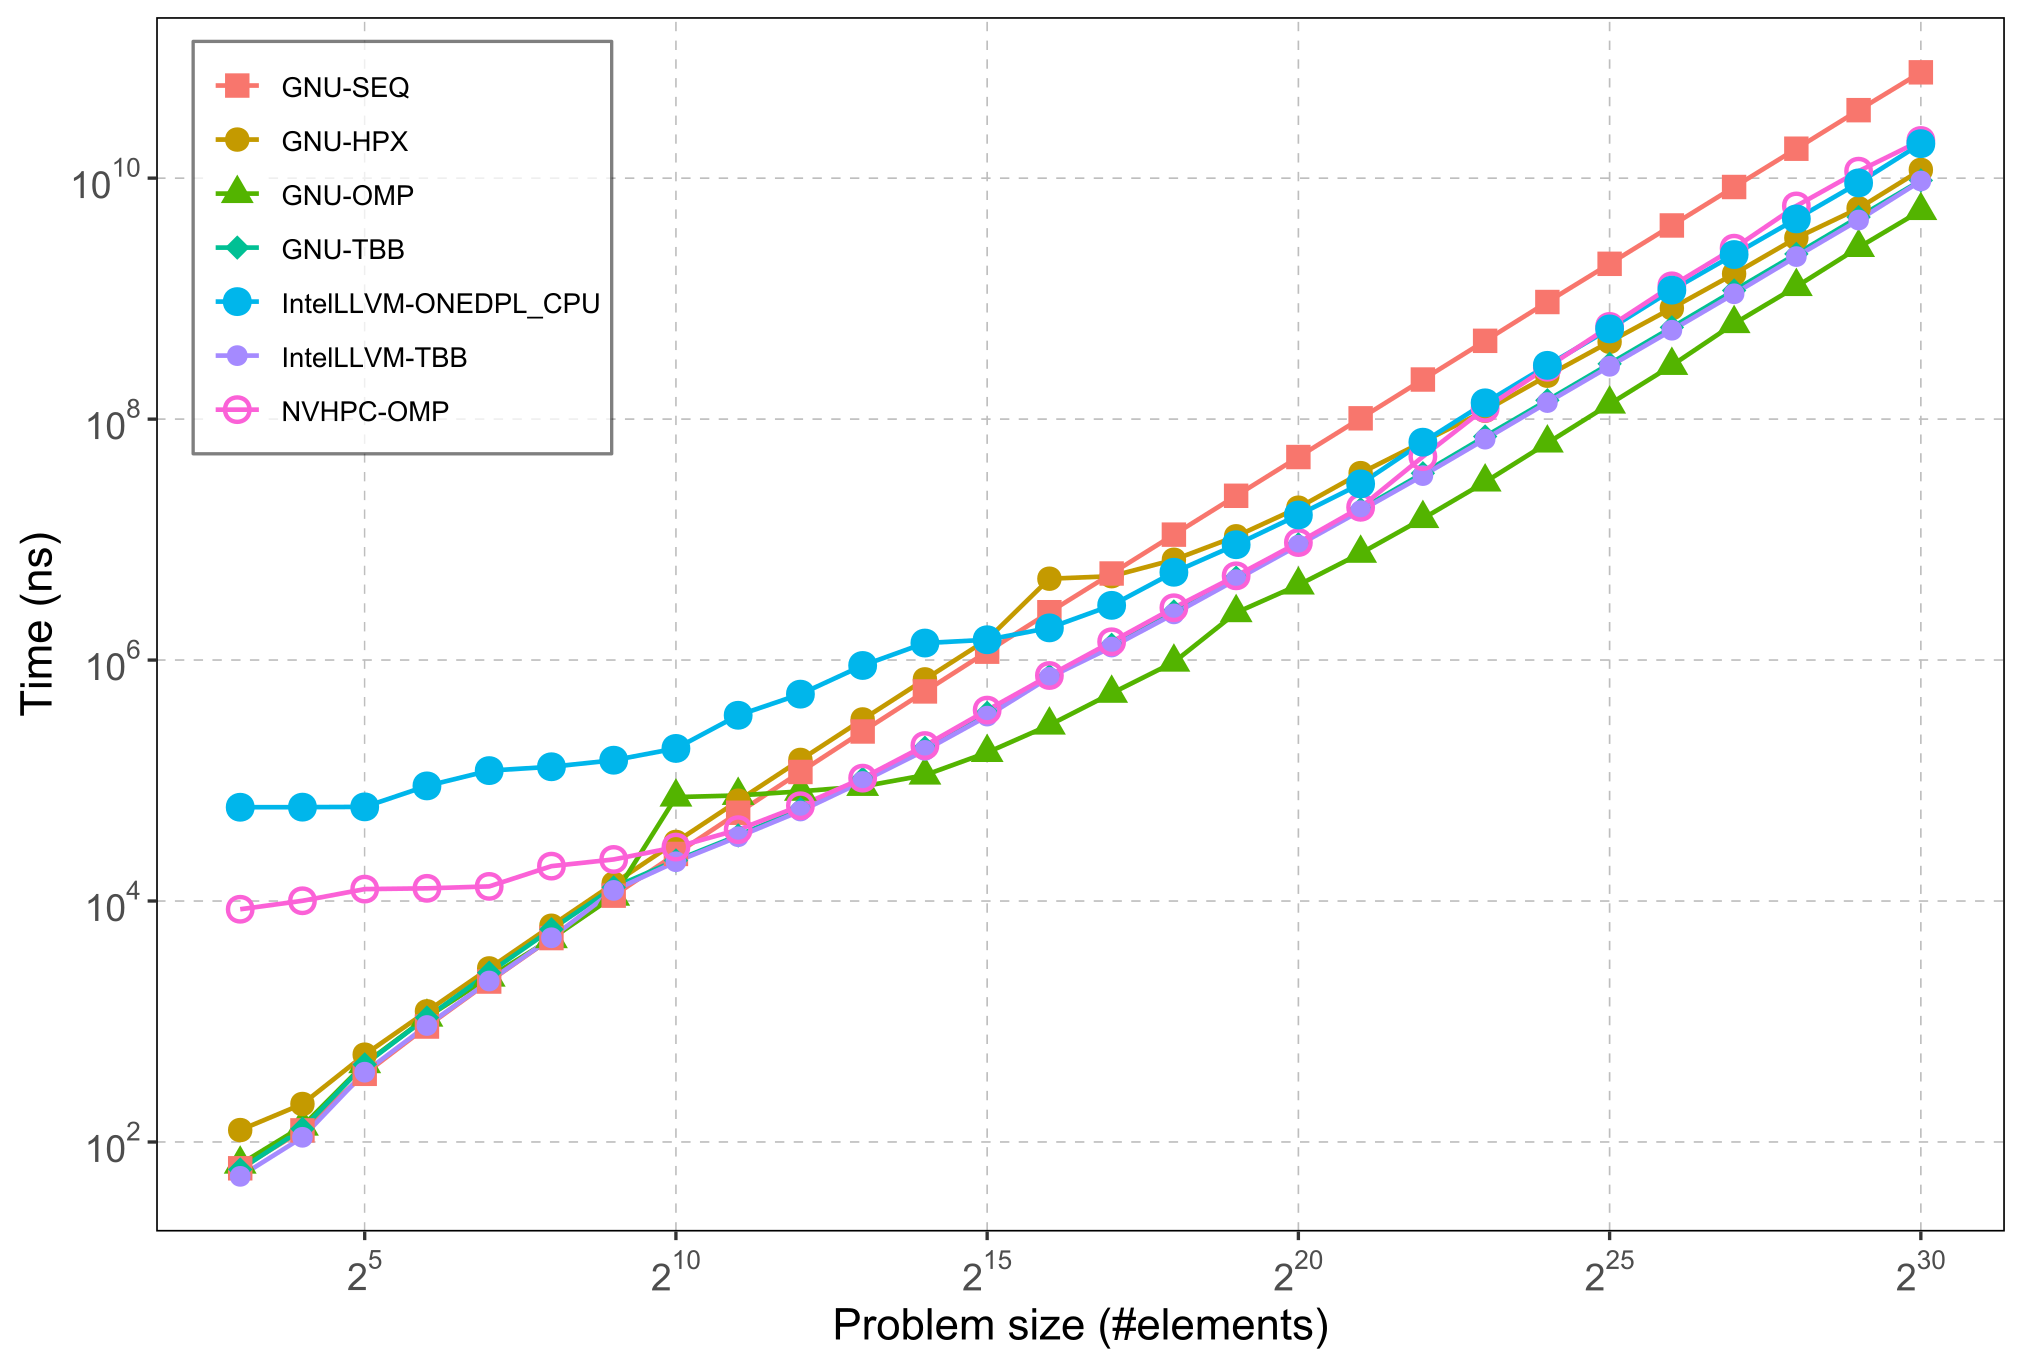
\includegraphics[width=\linewidth]{figures/problemSize_time-sort.png}
            \caption*{(a) Problem scaling. Lower is better.}
      \end{minipage}
      \hfill
      \begin{minipage}[t]{0.48\linewidth}
            \centering
            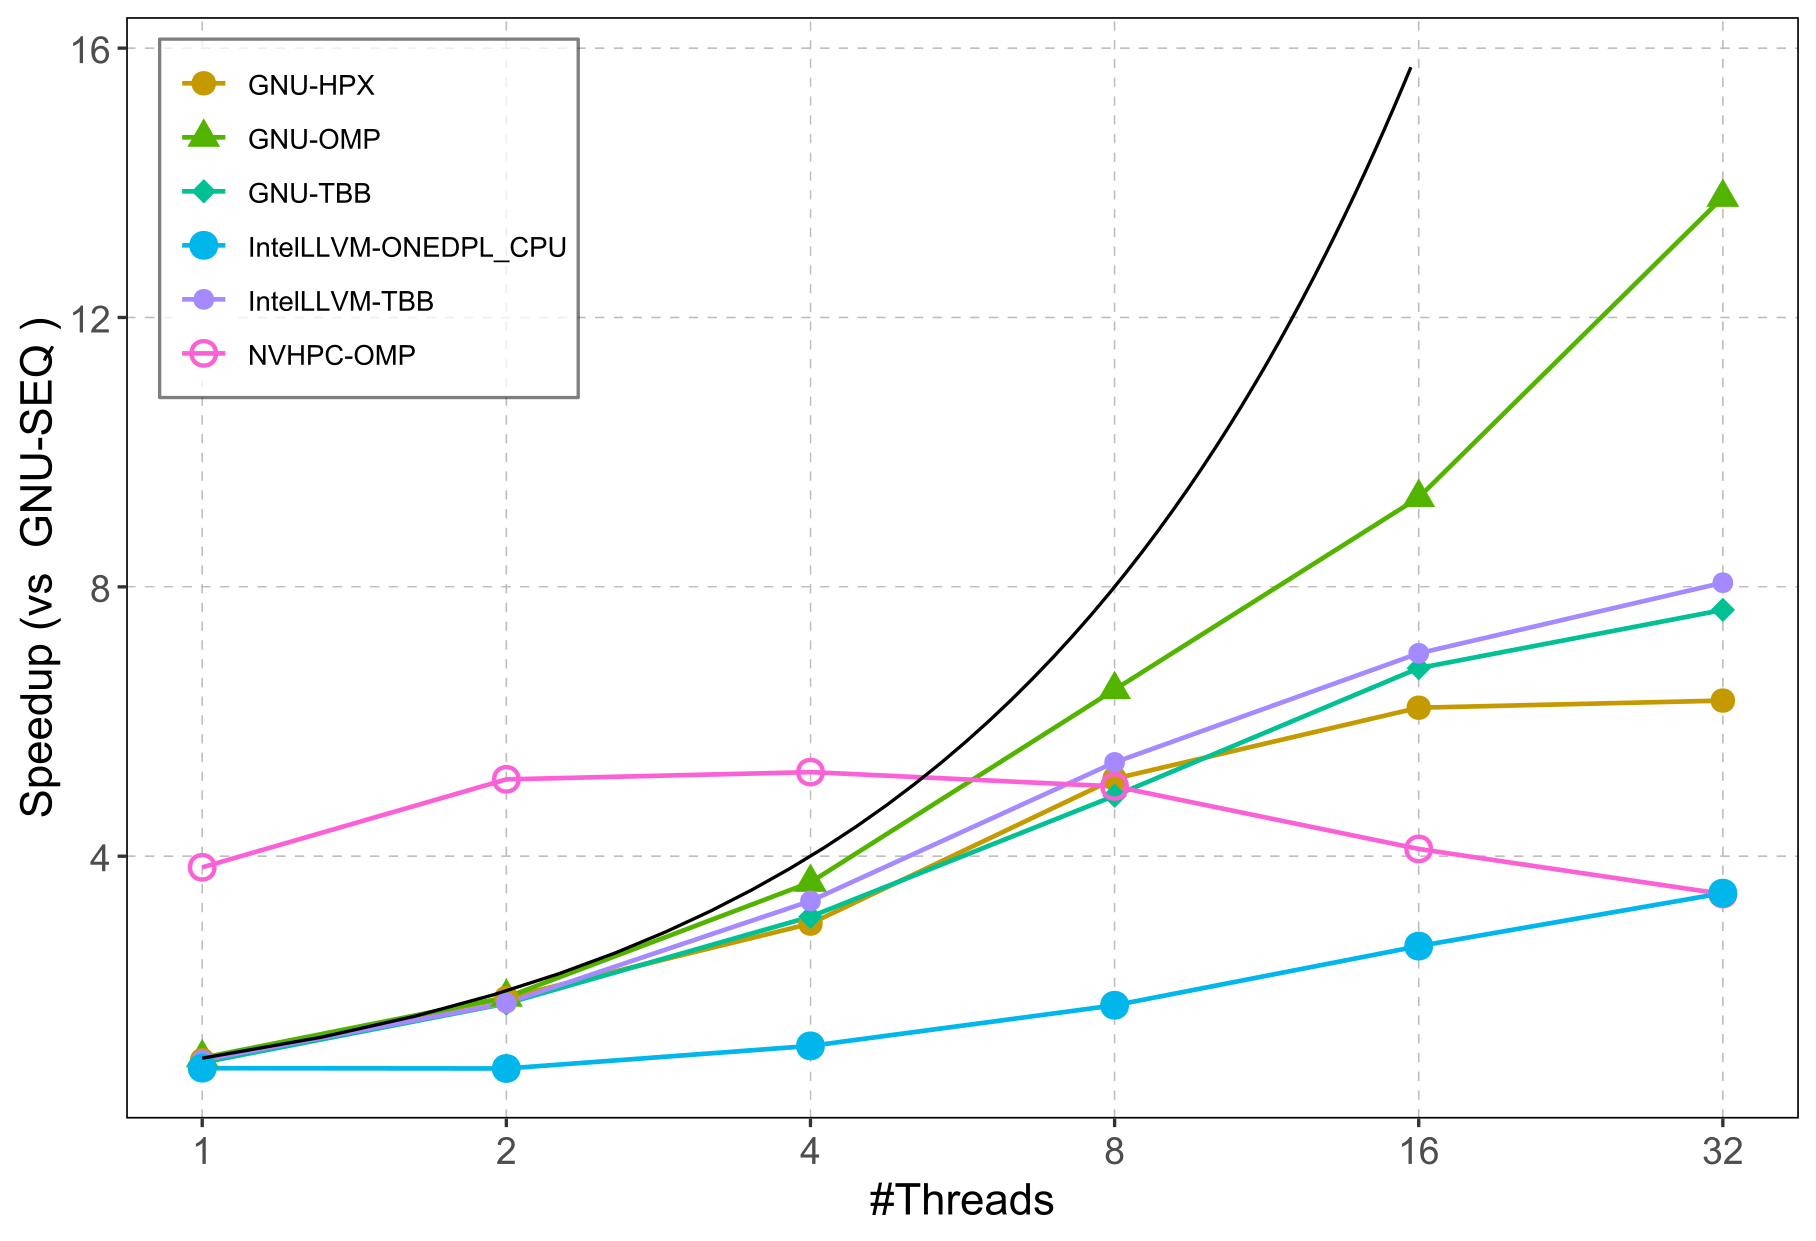
\includegraphics[width=\linewidth]{figures/speedup_threads-sort.png}
            \caption*{(b) Strong scaling with $2^{29}$ elements. Higher is better.}
      \end{minipage}
      \caption{Results for X::sort.}\label{fig:x::sort}
\end{figure}
\subsection{Summary of Results}

\mypar{Speedup}
Table~\ref{tab:summary_speedup} summarizes the experimental results, reporting
the maximum speedup achieved by each backend across the five parallel STL
algorithms. Speedup is shown for 8 and 32 threads to reflect the underlying
hardware architecture, which includes 8 performance cores (P-cores),
16 efficiency cores (E-cores), and 8 hyperthreads.

As observed in the original pSTL-Bench paper, all parallel implementations
outperform the sequential version across all algorithms. The average speedup
across all backends is approximately 3x.

Among the backends, oneDPL consistently achieved the lowest speedup but still
outperformed the sequential baseline in all algorithms except \textit{find} and
\textit{inclusive\_scan}.

\mypar{Efficiency}
Table~\ref{tab:summary_maxspeedup} reports the maximum number of threads for
which the efficiency—defined as
$\frac{\text{Speedup}}{\text{Number of Threads}}$—remains above 70\%
relative to sequential execution.

The results indicate that most backends maintain high efficiency up to 8
threads, which aligns with the processor's architecture, specifically the
presence of 8 performance cores.

\mypar{Binary Size}
Table~\ref{tab:summary_binary} presents the binary sizes generated by the
different compiler-backend combinations.

The results show considerable variation in binary size, with the oneDPL backend
on CPU producing the largest binaries. This is consistent with the complexity
of its implementation, which is generally more elaborate compared to the other
backends.

\begin{table*}[t]
      \centering
      \centering
      \caption{Speedup against GNU-SEQ sequential implementation with for 8 and 32 threads. Problem size is $2^{29}$. Higher is better.}\label{tab:summary_speedup}
      \begin{tabular}{l c c c c c c}
            \hline
            \textbf{Backend}      & \textbf{find} & \makecell{\textbf{for\_each}                                                   \\$k_{it}=1$} & \makecell{\textbf{for\_each}\\$k_{it}=1000$} & \textbf{inclusive\_scan} & \textbf{reduce} & \textbf{sort} \\
            \hline
            GNU-TBB               & 2.6 | 2.6     & 2.5 | 2.6                    & 6.0 | 17.3 & 1.2 | 1.2 & 3.0 | 3.0 & 4.8 | 7.6  \\
            GNU-OMP               & 2.8 | 2.6     & 2.4 | 2.6                    & 6.7 | 17.3 & N/A | N/A & 2.8 | 2.9 & 6.4 | 13.7 \\
            GNU-HPX               & 2.6 | 2.7     & 2.5 | 2.5                    & 5.9 | 17.4 & 1.2 | 1.2 & 3.0 | 3.0 & 5.1 | 6.3  \\
            IntelLLVM-TBB         & 2.7 | 2.6     & 2.5 | 2.6                    & 7.2 | 17.7 & 1.2 | 1.2 & 3.0 | 3.0 & 5.3 | 8.0  \\
            NVHPC-OMP             & 2.1 | 3.2     & 2.5 | 2.6                    & 6.2 | 12.6 & 1.0 | 1.0 & 3.0 | 3.0 & 5.0 | 3.4  \\
            IntelLLVM-ONEDPL\_CPU & 0.2 | 0.5     & 2.4 | 2.6                    & 2.4 | 6.9  & 0.5 | 0.6 & 2.4 | 2.8 & 1.7 | 3.4  \\
            \hline
      \end{tabular}
\end{table*}

\begin{table*}[t]
      \centering
      \centering
      \caption{Maximum number of threads such that efficiency = $\frac{\text{Speedup}}{\text{Number of Threads}}$ is above 70\% (compared to the seq. execution). Problem size is $2^{29}$. Higher is better.}\label{tab:summary_maxspeedup}
      \begin{tabular}{l c c c c c c}
            \hline
            \textbf{Backend}      & \textbf{find} & \makecell{\textbf{for\_each}                   \\$k_{it}=1$} & \makecell{\textbf{for\_each}\\$k_{it}=1000$} & \textbf{inclusive\_scan} & \textbf{reduce} & \textbf{sort} \\
            \hline
            GNU-TBB               & 1             & 2                            & 8 & N/A & 1 & 4 \\
            GNU-OMP               & 1             & 2                            & 8 & N/A & 1 & 8 \\
            GNU-HPX               & N/A           & 2                            & 8 & N/A & 2 & 4 \\
            IntelLLVM-TBB         & 2             & 2                            & 8 & N/A & 2 & 4 \\
            NVHPC-OMP             & N/A           & 2                            & 8 & 1   & 2 & 4 \\
            IntelLLVM-ONEDPL\_CPU & N/A           & 1                            & 1 & N/A & 2 & 2 \\
            \hline
      \end{tabular}
\end{table*}

\begin{table*}[t]
      \centering
      \centering
      \caption{ Binary sizes for the different compilers and backends used in the experiments. Lower is better.}\label{tab:summary_binary}
      \begin{tabular}{l c c c c c c c c c}
            \hline
            Compiler        & GNU & GNU & GNU & GNU & IntelLLVM & NVHPC & NVHPC & IntelLLVM   & IntelLLVM   \\
            Backend         & SEQ & TBB & OMP & HPX & TBB       & OMP   & CUDA  & ONEDPL\_CPU & ONEDPL\_GPU \\
            \hline
            Bin. size (MiB) & 0.9 & 1.9 & 0.9 & 4.1 & 3         & 1.6   & 8     & 30          & 18          \\
            \hline
      \end{tabular}
\end{table*}

\subsection{Performance on GPU}

This experiment focuses on the performance of parallel algorithms on GPU,
evaluated using the NVIDIA HPC SDK and oneDPL. All benchmarks are executed
using \textit{float} precision instead of \textit{double}, as GPUs are
traditionally more efficient with single-precision operations.

\mypar{for\_each}
Figure~\ref{fig:gpu_problemSize_time-for_each} shows the performance of the
\textit{for\_each} algorithm on GPU for two levels of arithmetic intensity:
$k_{it} = 1$ and $k_{it} = 1000$.

The results differ from those in the original pSTL-Bench paper. When the
arithmetic intensity is low ($k_{it} = 1$), GPU implementations previously
performed significantly worse than CPU implementations. In this evaluation,
however, the NVHPC-CUDA backend outperforms the sequential baseline, while the
oneDPL-GPU backend performs slightly worse.

When the arithmetic intensity is high ($k_{it} = 1000$), the results align more
closely with the original study. Both GPU backends outperform the sequential
version, with NVHPC-CUDA maintaining a clear advantage over oneDPL on GPU.

\begin{figure}[H]
      \centering
      \begin{minipage}[t]{0.48\linewidth}
            \centering
            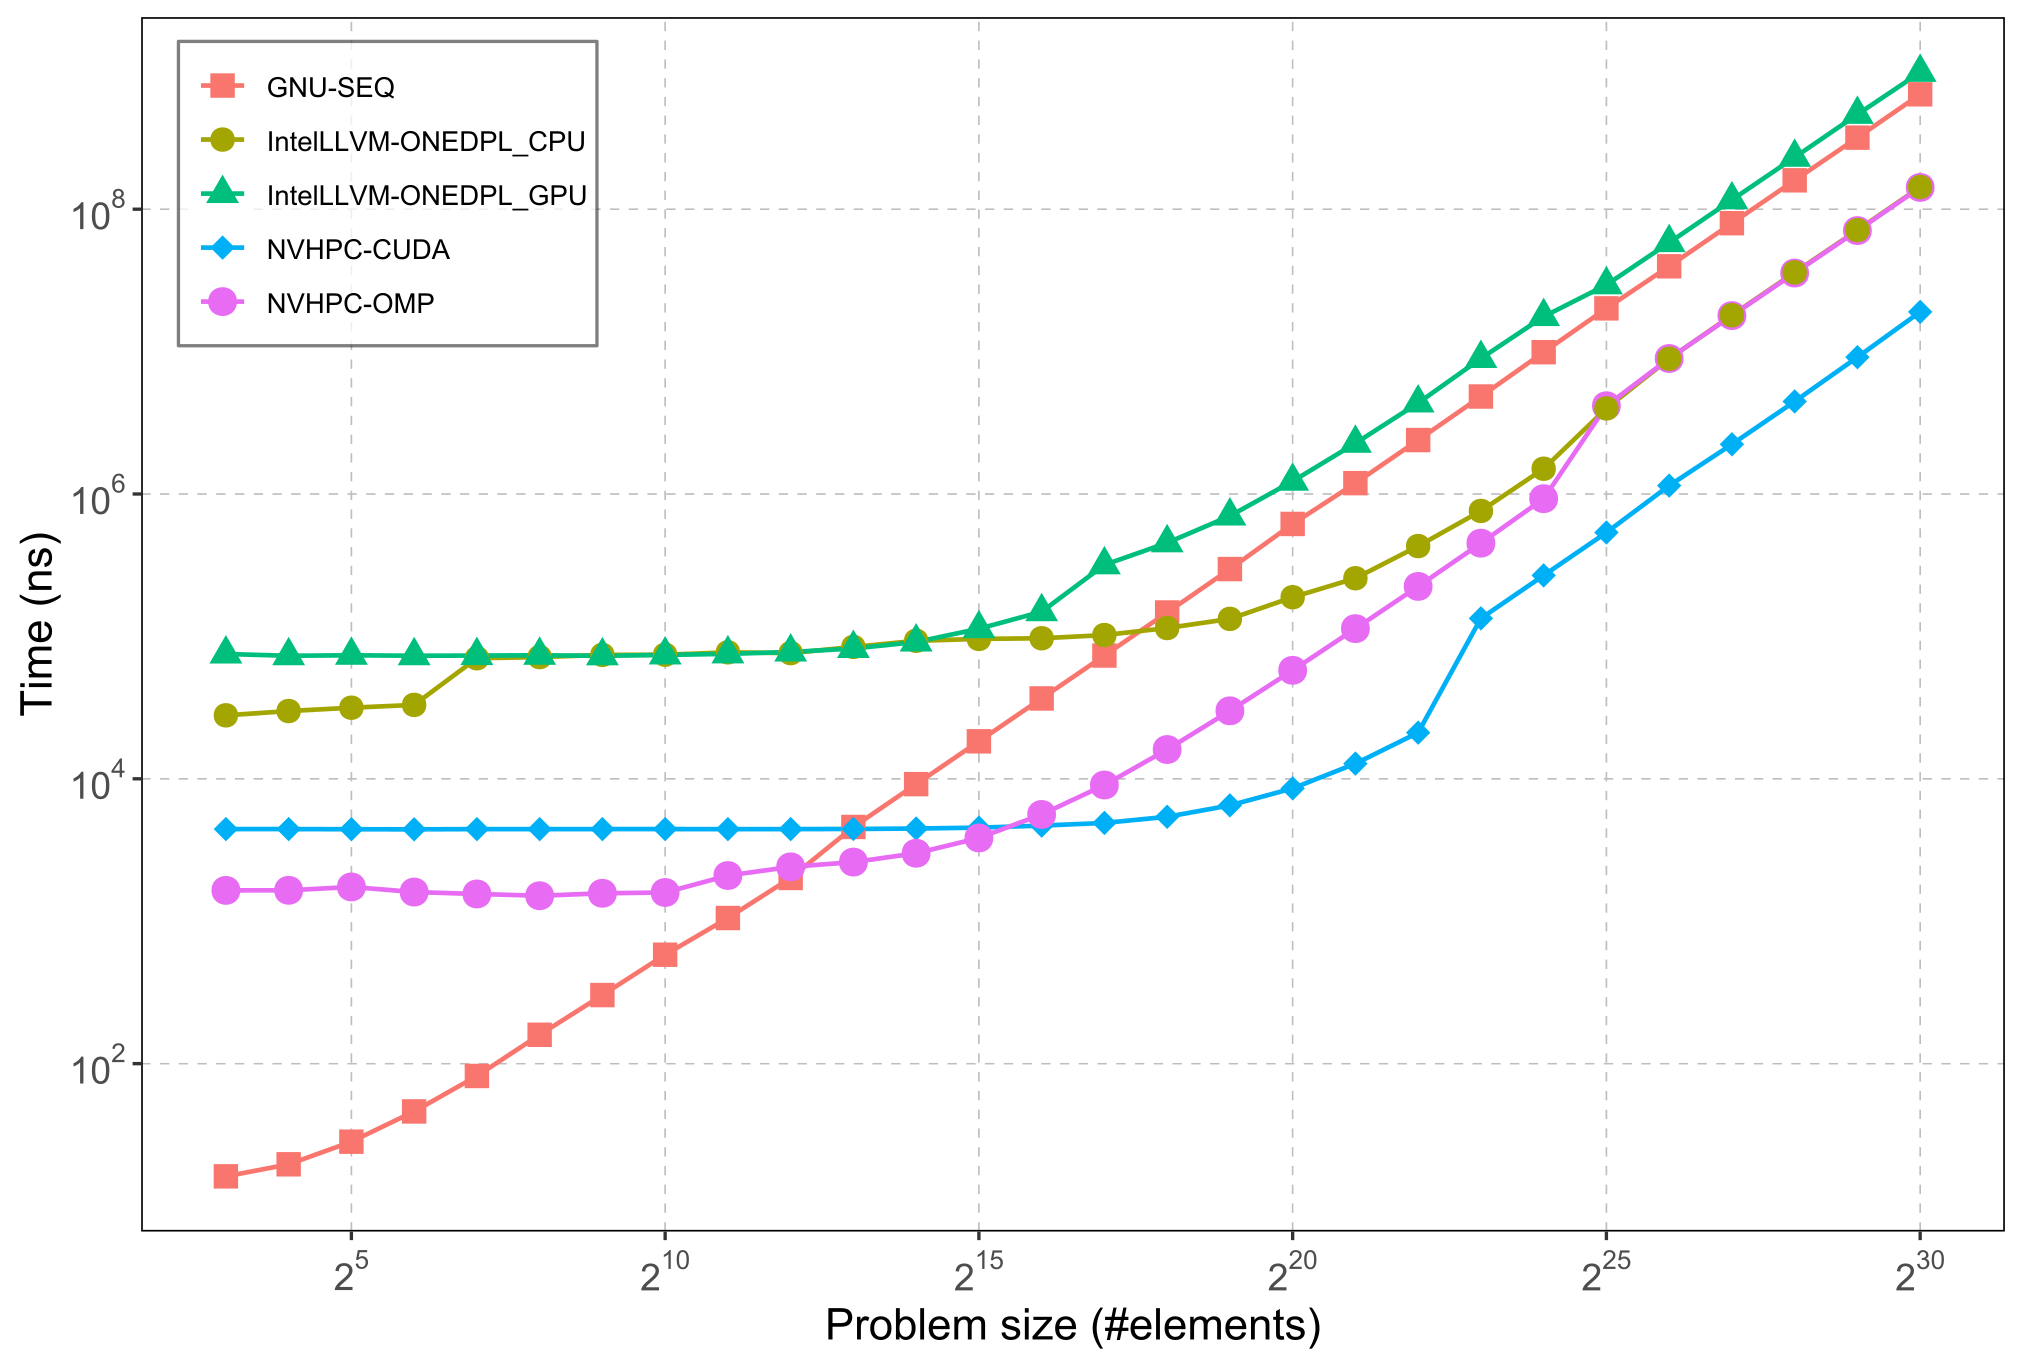
\includegraphics[width=\linewidth]{figures/gpu_problemSize_time-for_each-k1.png}
            \caption*{(a) $k_{it} = 1$.}
      \end{minipage}
      \hfill
      \begin{minipage}[t]{0.48\linewidth}
            \centering
            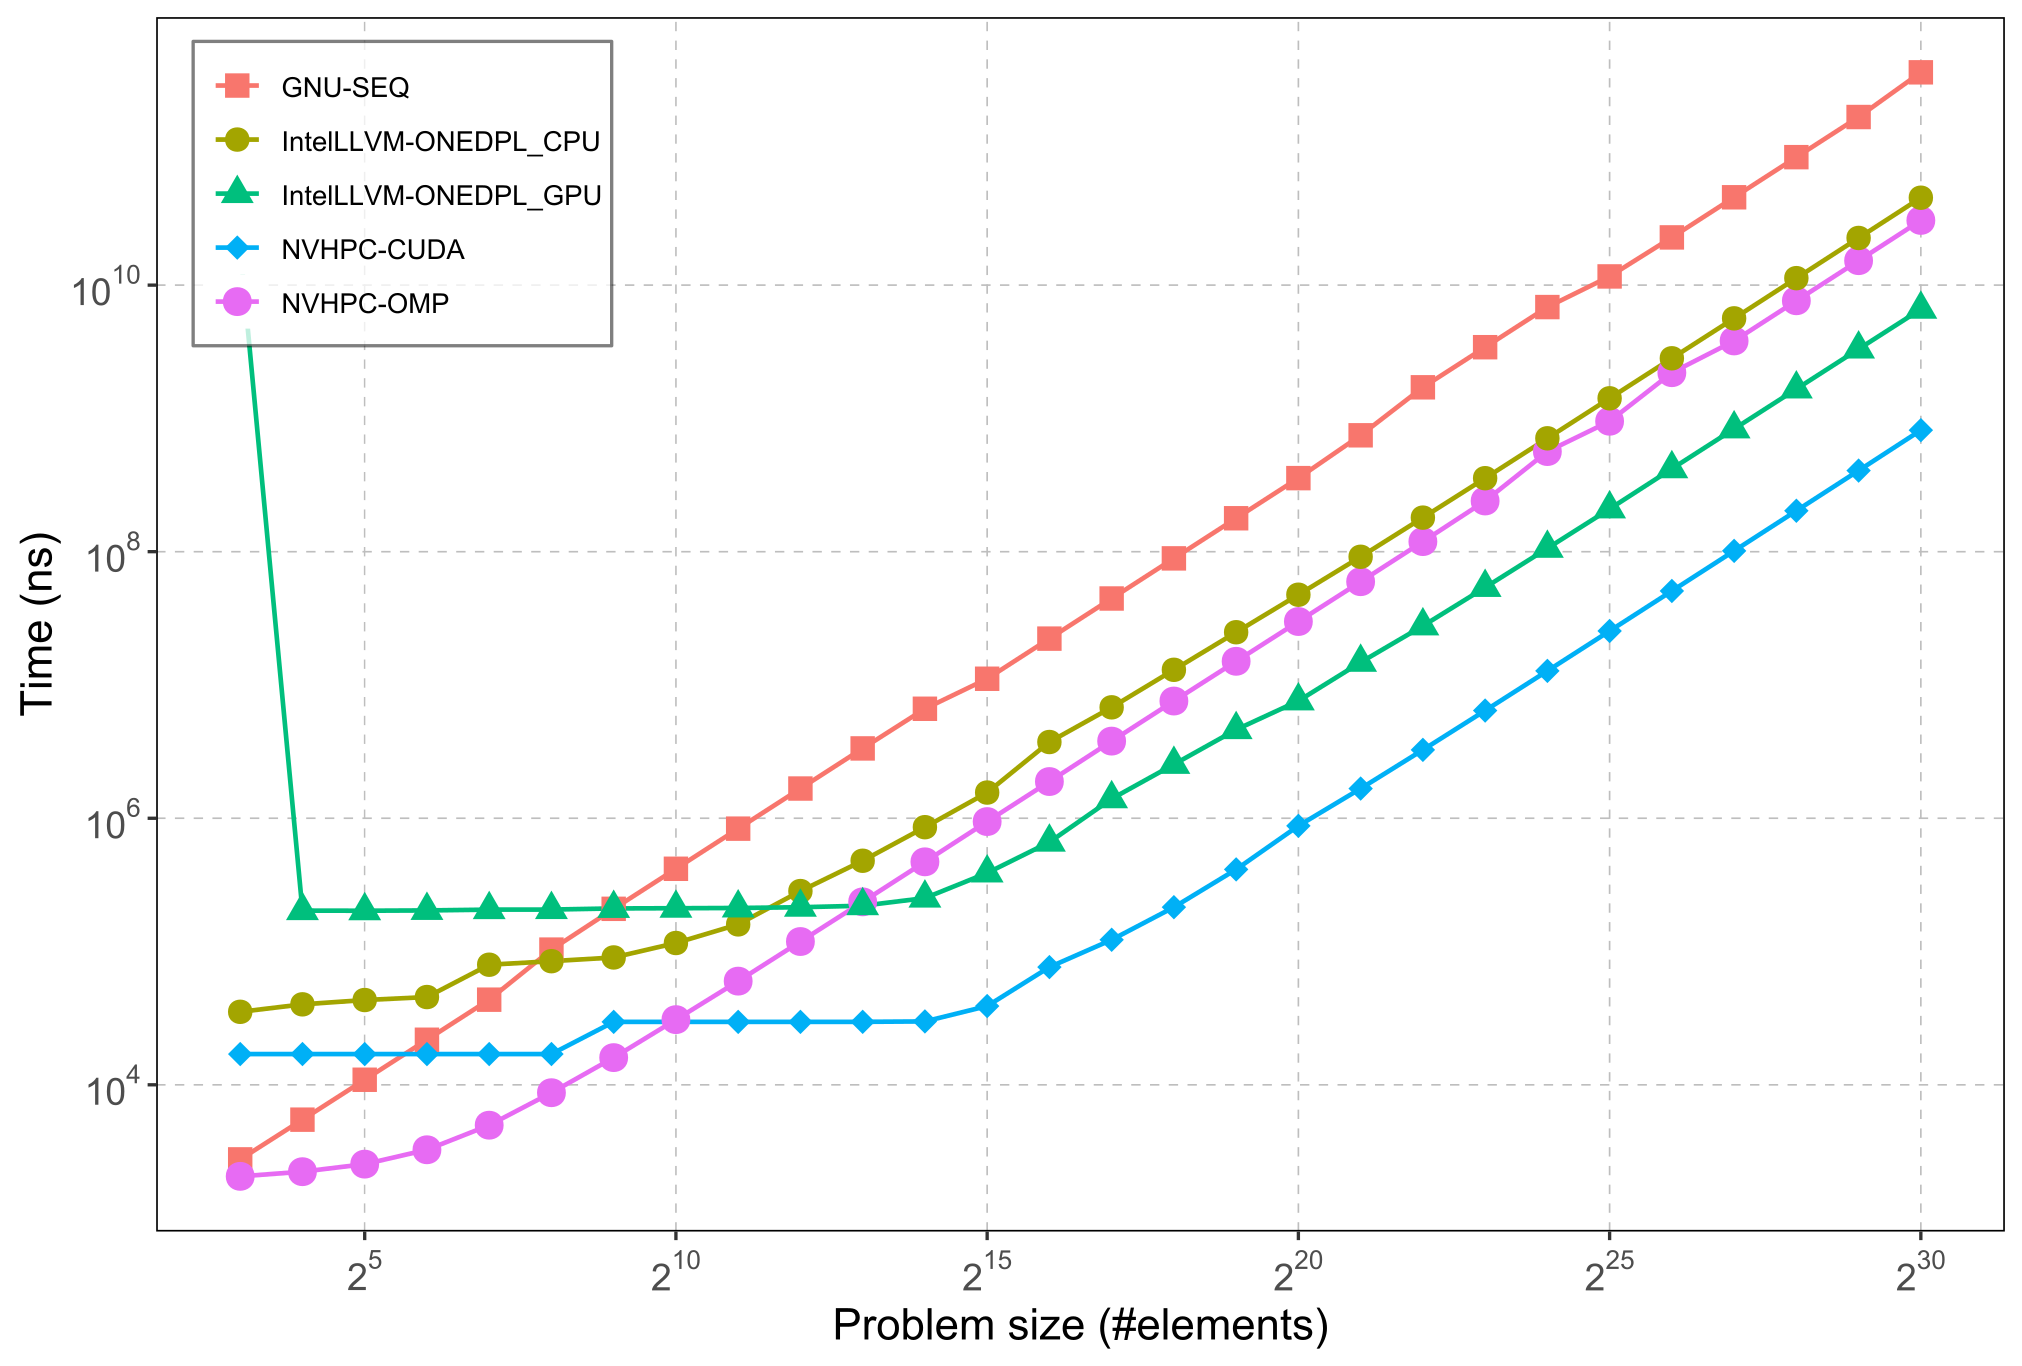
\includegraphics[width=\linewidth]{figures/gpu_problemSize_time-for_each-k1000.png}
            \caption*{(b) $k_{it} = 1000$.}
      \end{minipage}
      \caption{Results for X::for\_each. Problem scaling using all cores except for GNU-SEQ implementation.
            Data type: \textit{float}. Lower is better.}
      \label{fig:gpu_problemSize_time-for_each}
\end{figure}

\mypar{Float vs Double}
To evaluate the impact of data type on GPU performance, the \textit{for\_each}
benchmark with $k_{it} = 1000$ was executed using both \textit{float} and
\textit{double} types. The results are shown in
Figure~\ref{fig:gpu_float_vs_double}.

The NVHPC-CUDA backend shows a substantial performance gain when using
\textit{float}, highlighting the typical advantage of single-precision on GPUs.
In contrast, the oneDPL-GPU backend exhibits minimal difference between
\textit{float} and \textit{double}, indicating less sensitivity to data type.

\begin{figure}[H]
      \centering
      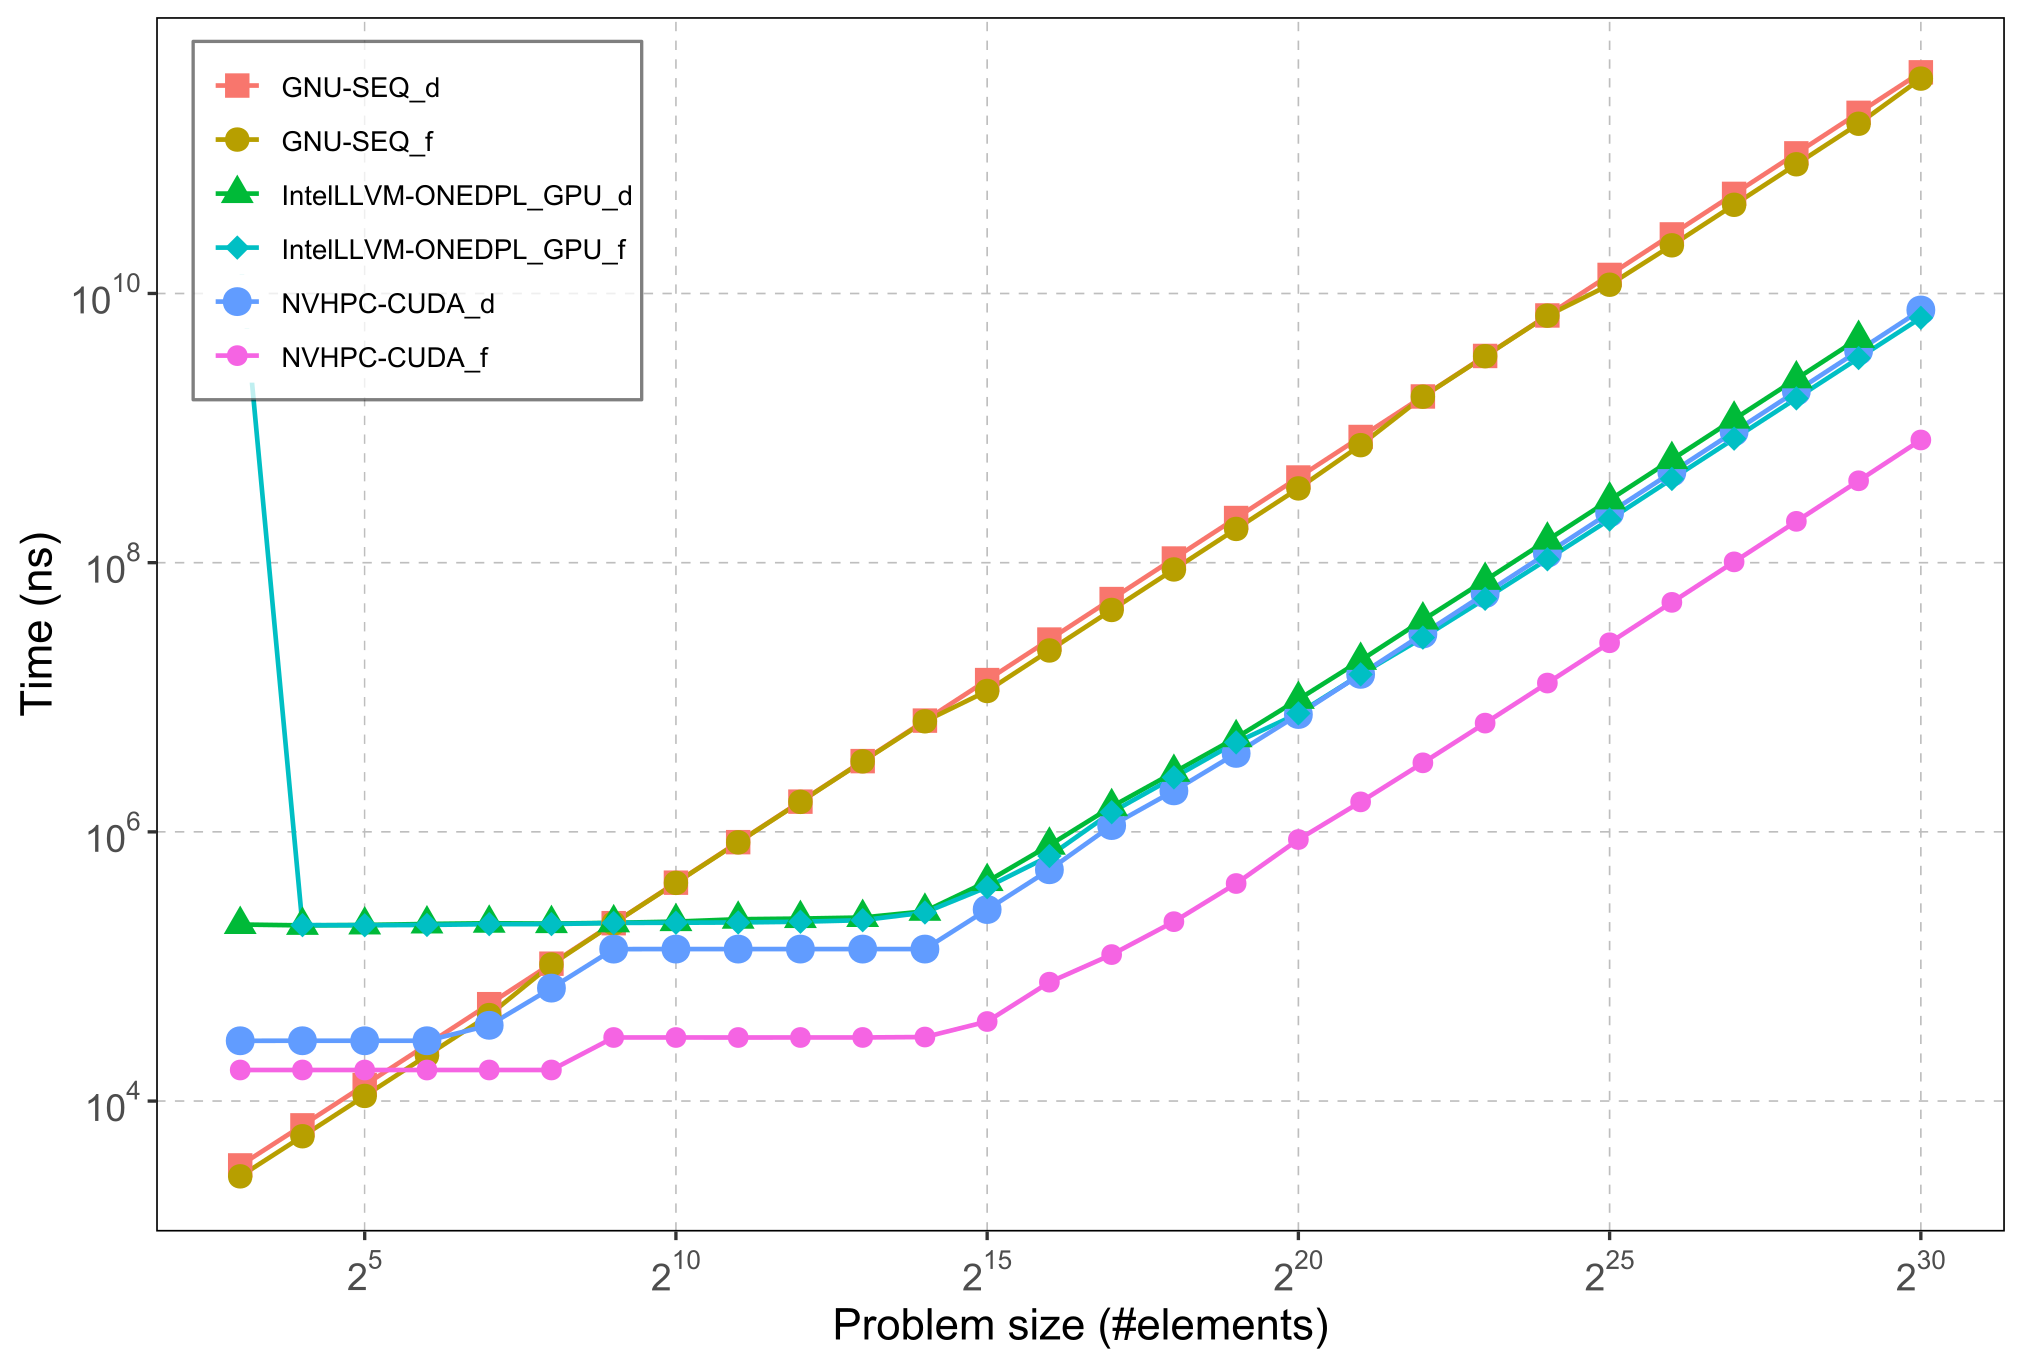
\includegraphics[width=\linewidth]{figures/gpu-floatVSDouble-problemSize_time-for_each-k1000.png}
      \caption{Performance comparison of \textit{for\_each} with $k_{it} = 1000$
            using \textit{float} and \textit{double}. Lower is better.}
      \label{fig:gpu_float_vs_double}
\end{figure}

\section{Conclusions}

This work reproduced and extended the pSTL-Bench benchmark to evaluate the
scalability of parallel STL implementations. The experiments were conducted
across a range of algorithms and execution backends, including CPU and GPU
platforms, with a particular focus on thread scaling, arithmetic intensity, and
hardware efficiency.

The results confirm that parallel STL implementations continue to outperform
their sequential counterparts, especially for compute-intensive workloads.
However, scalability is often limited by hardware constraints, such as the
heterogeneous core architecture found in modern CPUs. Most backends achieved
peak efficiency around 8 threads, which correlates with the number of
performance cores available.

The oneDPL backend on CPU consistently underperformed relative to other
implementations, particularly in memory-bound algorithms like \textit{find} and
\textit{inclusive\_scan}. On GPU, however, oneDPL delivered competitive results
at higher arithmetic intensities, although the NVHPC backend generally provided
better performance.

Additional experiments showed that GPU performance was significantly better
with \textit{float} precision compared to \textit{double}, especially for
NVHPC. This highlights the importance of considering data type and backend
capabilities when targeting heterogeneous platforms.

While the parallel STL is a viable and portable abstraction for parallelism,
its efficiency is highly dependent on compiler, backend, and hardware
characteristics. Developers aiming for high performance should carefully
evaluate these factors and selectively tune configurations based on target
architecture and workload characteristics.

\balance{}
\bibliographystyle{ACM-Reference-Format}
\begin{thebibliography}{1}

      \bibitem{pSTL-Bench_fork:github}
      ``Fork: pSTL-Bench: A Benchmark for Parallel STL Implementations'' \textit{GitHub Repository},
      \url{https://github.com/olegbilovus/pSTL-Bench}

      \bibitem{pSTL-Bench-report:github}
      ``Extending and Reproducing pSTL-Bench: oneDPL Backend Integration and Enhanced Reproducibility'' \textit{GitHub Repository},
      \url{https://github.com/olegbilovus/pSTL-Bench-report}

      \bibitem{pSTL-Bench}
      R. Laso, D. Krupitza, and S. Hunold, ``Exploring Scalability in C++ Parallel STL Implementations'' in \textit{Proceedings of the 53rd International Conference on Parallel Processing (ICPP '24)},
      Association for Computing Machinery, New York, NY, USA, 2024, pp. 284--293.
      \url{https://doi.org/10.1145/3673038.3673065}

      \bibitem{app}
      W. -C. Lin, T. Deakin and S. McIntosh-Smith, ``Evaluating ISO C++ Parallel Algorithms on Heterogeneous HPC Systems'' in  \textit{2022 IEEE/ACM International Workshop on Performance Modeling, Benchmarking and Simulation of High Performance Computer Systems (PMBS)},
      Dallas, TX, USA, 2022, pp. 36-47.
      \url{https://doi.org/10.1109/PMBS56514.2022.00009}

      \bibitem{Kokkos}
      H. C. Edwards and C. R. Trott, ``Kokkos: Enabling Performance Portability Across Manycore Architectures'' \textit{2013 Extreme Scaling Workshop (xsw 2013)},
      Boulder, CO, USA, 2013, pp. 18-24.
      \url{https://doi.org/10.1109/XSW.2013.7}

      \bibitem{RAJA}
      D. A. Beckingsale et al., ``RAJA: Portable Performance for Large-Scale Scientific Applications'' \textit{2019 IEEE/ACM International Workshop on Performance, Portability and Productivity in HPC (P3HPC)},
      Denver, CO, USA, 2019, pp. 71-81.
      \url{https://doi.org/10.1109/P3HPC49587.2019.00012}

      \bibitem{cpu_specs}
      Intel, ``Intel Core i9-13900HX Processor'' \textit{Intel SKU},
      \url{https://www.intel.com/content/www/us/en/products/sku/232171/intel-core-i913900hx-processor-36m-cache-up-to-5-40-ghz/specifications.html}

      \bibitem{gpu_specs}
      NVIDIA, ``GeForce RTX 4070 Laptop GPU'' \textit{GeForce RTX 40 Series Laptops},
      \url{https://www.nvidia.com/en-us/geforce/laptops/40-series/}

      \bibitem{google_benchmark:governor}
      Google Benchmark, ``Reducing Variance, Disabling CPU Frequency Scaling'' \textit{Google Benchmark Documentation},
      \url{https://google.github.io/benchmark/reducing_variance.html}

\end{thebibliography}

\end{document}

